\documentclass[
	% -- opções da classe memoir --
	12pt,				% tamanho da fonte
	openright,			% capítulos começam em pág ímpar (insere página vazia caso preciso)
	oneside,			% para impressão em recto e verso. Oposto a oneside
	a4paper,			% tamanho do papel. 
	% -- opções da classe abntex2 --
	%chapter=TITLE,		% títulos de capítulos convertidos em letras maiúsculas
	%section=TITLE,		% títulos de seções convertidos em letras maiúsculas
	%subsection=TITLE,	% títulos de subseções convertidos em letras maiúsculas
	%subsubsection=TITLE,% títulos de subsubseções convertidos em letras maiúsculas
	% -- opções do pacote babel --
	english,			% idioma adicional para hifenização
	brazilian				% o último idioma é o principal do documento
	]{abntex2}
\setlength{\headheight}{29pt}

% ---
% Pacotes acrescentados
% \usepackage{arydshln}
\usepackage{seqsplit}
\usepackage{rotating}

\usepackage{multirow}
%\usepackage[boxruled,linesnumbered,portuguese]{algorithm2e}

\usepackage{tabularray}
\usepackage{verbatim}

\usepackage{algpseudocode}



\usepackage{tikz}
\usetikzlibrary{shapes.geometric, arrows, positioning}

% Definição de estilos
\tikzstyle{startstop} = [rectangle, rounded corners, minimum width=3cm, minimum height=1cm,text centered, draw=black, fill=red!30]
\tikzstyle{process} = [rectangle, minimum width=3cm, minimum height=1cm, text centered, draw=black, fill=orange!30]
\tikzstyle{decision} = [diamond, minimum width=3cm, minimum height=1cm, text centered, draw=black, fill=green!30]
\tikzstyle{arrow} = [thick,->,>=stealth]

% -------------------------
%%----------------------------------------------------------------------------------
%% DEFINIÇÃO DE COMANDOS - adicionado 10/2020 - Modelo Willian
%%----------------------------------------------------------------------------------
\usepackage{rotating}				% Usado para rotacionar tabela
\usepackage[table]{xcolor}			% Cores em tabelas
\usepackage{caption}
%%\usepackage{subcaption}
\usepackage[skip=0.5ex]{subcaption}


% Reduz a fonte das legendas de figuras e tabelas
\captionnamefont{\small}
\captiontitlefont{\small}


% Conteúdo da tabela
\newcommand{\cell}[1]{{\ttfamily \scriptsize #1}}

\newcommand{\imgref}[1]{%
	\begin{minipage}[h][1.8\fontcharwd\font`\B][c]{1.8\fontcharht\font`\B}%
		%\centering%
		%\vfill%
		\includegraphics[height=1.7\fontcharht\font`\B]{images/#1.eps}%
		%\vfill%
	\end{minipage}%
}

%
%\usepackage{algorithm}
%\usepackage{algorithmic}

% ---
% Pacotes básicos 
% ---
\usepackage{lmodern}			% Usa a fonte Latin Modern			
\usepackage[T1]{fontenc}		% Selecao de codigos de fonte.
\usepackage[utf8]{inputenc}		% Codificacao do documento (conversão automática dos acentos)

\usepackage{lastpage}			% Usado pela Ficha catalográfica
\usepackage{indentfirst}		% Indenta o primeiro parágrafo de cada seção.
\usepackage{color}				% Controle das cores
\usepackage{url}				% Citar URLs
\usepackage{graphicx}	
\usepackage{enumitem}
\newcolumntype{Y}{>{\raggedright\arraybackslash}X}

% Lista compacta dentro de célula
\newcommand{\cellitemize}[1]{%
\begin{minipage}[t]{\hsize}\vspace{0pt}\raggedright
\begin{itemize}[leftmargin=1.2em,labelsep=0.4em,itemsep=0pt,topsep=0pt,parsep=0pt,partopsep=0pt]
#1
\end{itemize}
\end{minipage}%
}

\newcolumntype{P}[1]{>{\raggedright\arraybackslash}p{#1}}
\newcommand{\tabitem}{\textbullet\ }
% Inclusão de gráficos
\graphicspath{ {img/} }

%vide link - dois comandos abaixo
%https://subscription.packtpub.com/book/business-and-other/9781801078658/2/ch02lvl1sec15/breaking-lines-and-paragraphs
%\usepackage{microtype}
%\usepackage[none]{hyphenat}
\usepackage{microtype} 			% para melhorias de justificação

\usepackage{multirow}
\usepackage{varwidth} %for the varwidth minipage environment out/2020
% ---
		
% ---
% Pacotes adicionais, usados apenas no âmbito do Modelo Canônico do abnteX2
% ---
\usepackage{lipsum}				% para geração de dummy text
\usepackage{amssymb}			% para uso de símbolos matemáticos
% ---

% ---
% Pacotes de citações
% ---
\usepackage[brazilian,hyperpageref]{backref}	 % Paginas com as citações na bibl
\usepackage[alf]{abntex2cite}	% Citações padrão ABNT

% Pacotes adicionais Matheus
\usepackage{array}
%\usepackage{soul}
%\usepackage{tablefootnote}
\usepackage{afterpage}
\usepackage{pdflscape}
%\newcolumntype{P}[1]{>{\centering\arraybackslash}p{#1}} % comentado 10/2020
\usepackage{amsmath}
%\usepackage{algorithm} % comentado contado 30/04/2020
\usepackage[portuguese, ruled, linesnumbered]{algorithm2e} % incluido
\usepackage{adjustbox} % max width=\textwidth
\usepackage{booktabs}
% Tabelas longas

% Tabelas com linhas profissionais: \toprule, \midrule, \bottomrule

% Para criar coluna P{...}

% Coluna P com alinhamento à esquerda e quebra automática de linha
%% Adicionado por Cláudio para usar \citet
%\usepackage{natbib}
%\bibliographystyle{plainnat}
\usepackage{longtable}
\usepackage{makecell}
\usepackage{tabularx}
% Fim da adição
\usepackage{float}
\usepackage{forest}
%\usepackage{algpseudocode}
\usepackage{listings} % Para inclusao de codigos fontes
\usepackage{xltabular} % quebra página + coluna X
\usepackage{color}
%\definecolor{gray}{rgb}{0.8,0.8,0.8}
\definecolor{gray}{gray}{0.8}
\lstset{ %
	backgroundcolor=\color{white},   % choose the background color; you must add \usepackage{color} or \usepackage{xcolor}
	basicstyle=\footnotesize,        % the size of the fonts that are used for the code
	breakatwhitespace=false,         % sets if automatic breaks should only happen at whitespace
	breaklines=true,                 % sets automatic line breaking
	captionpos=t,                    % sets the caption-position to bottom
	commentstyle=\color{mygreen},    % comment style
	deletekeywords={...},            % if you want to delete keywords from the given language
	escapeinside={\%*}{*)},          % if you want to add LaTeX within your code
	extendedchars=true,              % lets you use non-ASCII characters; for 8-bits encodings only, does not work with UTF-8
	frame=single,	                   % adds a frame around the code
	keepspaces=true,                 % keeps spaces in text, useful for keeping indentation of code (possibly needs columns=flexible)
	keywordstyle=\color{blue},       % keyword style
	language=Octave,                 % the language of the code
	otherkeywords={*,...},           % if you want to add more keywords to the set
	numbers=left,                    % where to put the line-numbers; possible values are (none, left, right)
	numbersep=5pt,                   % how far the line-numbers are from the code
	numberstyle=\tiny\color{mygray}, % the style that is used for the line-numbers
	rulecolor=\color{black},         % if not set, the frame-color may be changed on line-breaks within not-black text (e.g. comments (green here))
	showspaces=false,                % show spaces everywhere adding particular underscores; it overrides 'showstringspaces'
	showstringspaces=false,          % underline spaces within strings only
	showtabs=false,                  % show tabs within strings adding particular underscores
	stepnumber=1,                    % the step between two line-numbers. If it's 1, each line will be numbered
	stringstyle=\color{mymauve},     % string literal style
	tabsize=2,	                   % sets default tabsize to 2 spaces
	title=\lstname,                   % show the filename of files included with \lstinputlisting; also try caption instead of title
	numberbychapter=false
}
\renewcommand\lstlistingname{Script}
%Alteração Rondado - as linhas abaixo foram comentandas
%\renewcommand{\listalgorithmname}{Lista de Algoritmos}
%\renewcommand{\listalgorithmname}{Lista de Algoritmos}
%\renewcommand{\lstlistlistingname}{Lista de Scripts}
%\floatname{algorithm}{Algoritmo}

%fim alteração

%\usepackage[T1]{fontenc}
%\usepackage[scaled]{beramono}
%\usepackage{listings}
%\lstset{
%	language=Python,
%	showstringspaces=false,
%	formfeed=newpage,
%	tabsize=1,
%	commentstyle=itshape,
%	basicstyle=ttfamily,
%	stepnumber=1,
%	morekeywords={models, lambda, forms}
%}

% ---


% --- 
% CONFIGURAÇÕES DE PACOTES
% --- 

%\hyphenation{a-di-cio-nal-men-te}

% ---
% Configurações do pacote backref
% Usado sem a opção hyperpageref de backref
\renewcommand{\backrefpagesname}{Citado na(s) página(s):~}
% Texto padrão antes do número das páginas
\renewcommand{\backref}{}
% Define os textos da citação
\renewcommand*{\backrefalt}[4]{
	\ifcase #1 %
		Nenhuma citação no texto.%
	\or
		Citado na página #2.%
	\else
		Citado #1 vezes nas páginas #2.%
	\fi}%
% ---

%-----
%Adaptações do formato ABNT para UNESP
\addto\captionsbrazil{
	\renewcommand{\listfigurename}{Lista de Figuras}
	\renewcommand{\listtablename}{Lista de Tabelas}
	\renewcommand{\listadesiglasname}{Lista de Abreviaturas e Siglas}
	%\renewcommand{\folhadeaprovacaoname}{Folha de Aprovação}
	\renewcommand{\listadesimbolosname}{Lista de Símbolos}
}
%-----



%Comandos para padronização - Matheus
\newcommand{\suporte}{\textit{suporte}}
\newcommand{\confianca}{\textit{confiança}}
\newcommand{\itemset}{\textit{itemset}}
\newcommand{\itemsets}{\textit{itemsets}}
\newcommand{\kitemset}{\textit{k-itemset}}
\newcommand{\kitemsets}{\textit{k-itemsets}}
\newcommand{\nitemset}[1]{\textit{#1-itemset}}
\newcommand{\nitemsets}[1]{\textit{#1-itemsets}}
\newcommand{\apriori}{\textit{Apriori }}
\newcommand{\cl}{\textit{Clustering}}
\newcommand{\sky}{\textit{Sky}}
%\newcommand{\ABNTEXfontereduzidaTiny}{\tiny}
%\newcommand{\ABNTEXfontereduzidaScriptsize}{\scriptsize}
%\newcommand{\ABNTEXfontereduzidaSmall}{\small}

\usepackage{ragged2e}
\newcolumntype{L}[1]{>{\RaggedRight\arraybackslash}p{#1}}



% ---
% Configurações de aparência do PDF final

% alterando o aspecto da cor azul
\definecolor{blue}{RGB}{41,5,195}

%veronica: adicionei
\usepackage{hyperref}

% informações do PDF
\makeatletter
%veronica: aqui que muda a cor do hyperlink
\hypersetup{
     	%pagebackref=true,
		pdftitle={\@title}, 
		pdfauthor={\@author},
    	pdfsubject={\imprimirpreambulo},
	    pdfcreator={regras de associação},
		pdfkeywords={regras de associação}{mineração de dados}{trabalho de conclusão de curso}{unesp}, 
		colorlinks=true,       		% false: boxed links; true: colored links
    	linkcolor=blue,          	% color of internal links
    	citecolor=blue,        		% color of links to bibliography
    	filecolor=magenta,      		% color of file links
		urlcolor=blue,
		bookmarksdepth=4
}
\makeatother
% --- 

% --- 
% Espaçamentos entre linhas e parágrafos 
% --- 

% O tamanho do parágrafo é dado por:
\setlength{\parindent}{1.3cm}

% Controle do espaçamento entre um parágrafo e outro:
\setlength{\parskip}{0.2cm}  % tente também \onelineskip

% ---
% compila o indice
% ---
\makeindex
% ---
\DeclareMathOperator*{\median}{median}
% ----
% Início do documento
% ----
\begin{document}
% ---
% Informações de dados para CAPA e FOLHA DE ROSTO
% ---
%Mineração de Dados Temporais na Tarefa de Alocação Orçamentária: Um Estudo Exploratório
\titulo{Estratégias de Ensemble para Seleção de \\ Atributos em Classificação Associativa}
\autor{Vinícius de Souza Santos}
\local{Rio Claro - SP}
\data{2026}
\orientador[Orientadora:]{Profa. Dra. Veronica Oliveira de Carvalho}
\instituicao{ \center
	\vspace*{0.5mm}
	\begin{minipage}{0.3\textwidth}
		
\includegraphics[width=\textwidth]{figuras/unesplogo.pdf}
	\end{minipage}
	\hspace{1ex}
	\begin{minipage}{0.6\textwidth}
		\fontsize{12}{12}\selectfont \textbf{
			UNIVERSIDADE ESTADUAL PAULISTA\\
			``JÚLIO DE MESQUITA FILHO''\\
			{\small\hspace*{2mm}Câmpus de Rio Claro}}
	\end{minipage}
	
	\vspace*{3cm}}

%Mineração de Dados Temporais na Tarefa de Alocação Orçamentária: Um Estudo Exploratório
\tipotrabalho{Estratégias de Ensemble para Seleção de \\ Atributos em Classificação Associativa}
% O preambulo deve conter o tipo do trabalho, o objetivo, 
% o nome da instituição e a área de concentração 
\preambulo{Monografia apresentada ao Programa de Pós-graduação em Ciência da Computação – área de Inteligência Computacional, para o Exame de Qualificação, como parte dos requisitos para a obtenção do título de Mestre em Ciência da Computação.}
% ---

% Seleciona o idioma do documento (conforme pacotes do babel)
%\selectlanguage{english}
\selectlanguage{brazil}

% Retira espaço extra obsoleto entre as frases.
\frenchspacing 

% ----------------------------------------------------------
% ELEMENTOS PRÉ-TEXTUAIS
% ----------------------------------------------------------

\pretextual



\begin{capa}%
	\begin{center}
	\Large\imprimirinstituicao
	\end{center}

	\begin{center}
%	\vspace*{3.0cm}
	\Large Vinícius de Souza Santos
	\vspace*{3.0cm}
	
	\Large \textbf{\imprimirtitulo}
	
	\vspace*{3.0cm}
	
%	\noindent Orientadora: Profa. Dra. Veronica Oliveira de Carvalho
	
	\vspace*{6.0cm}
	
	{\large\imprimirlocal}
	\vspace*{-4mm}
	\par
	{\large\imprimirdata}
	 \vspace*{1cm}
	\end{center}
  \end{capa}


\begin{folhaderosto}
	\begin{center}		
		\fontsize{14}{14}\selectfont Vinícius de Souza Santos
		\vspace*{\fill}\vspace*{\fill}
		\begin{center}
			\ABNTEXchapterfont\bfseries\Large\imprimirtitulo
		\end{center}
		\vspace*{\fill}
		
		\hspace{.45\textwidth}
		\begin{minipage}{.5\textwidth}
			\SingleSpacing
			\imprimirpreambulo
		\end{minipage}%		
		
	 %	\vspace*{1cm}
	 %	\begin{flushright}
	%		\noindent Aluno: Maicon Dall'Agnol
	%	\end{flushright}
		\vspace*{1cm}
		\begin{flushright}
			\noindent Orientadora: Profa. Dra. Veronica Oliveira de Carvalho
		\end{flushright}
		\vspace*{1cm}
				
				
		{\large\imprimirlocal}
		\par
		{\large\imprimirdata}
		\vspace*{1cm}
		
	\end{center}
\end{folhaderosto}


\underline{}% ----------------------------------------------------------
% Resumo
% ----------------------------------------------------------
\chapter*{Resumo}\label{resumo}
% ----------------------------------------------------------

%Ranqueamento em Classificadores Associativos através da Agregação de Medidas Objetivas

A mineração de dados é o processo de descobrir padrões e conhecimentos a partir de grandes quantidades de dados objetivando analisar padrões frequentes e correlações contidas nos dados, com especial interesse em padrões inesperados, envolvendo assim um conjunto de métodos e técnicas. Apesar dessas técnicas já estarem bem difundidas em diversos setores da sociedade, percebe-se grande potencial de utilização a ser desenvolvido no setor público, em especial na área de orçamentação pública.  
Neste contexto, este trabalho se propõe a avaliar o uso de técnicas de inteligência computacional no campo do orçamento público de forma geral e, especificamente, na tarefa específica de previsão das despesas orçamentárias.

\textbf{Palavras-chaves:} mineração de dados; aprendizado de máquina; orçamento público.

%\par


%\chapter*{Abstract}\label{Abstract}
% ----------------------------------------------------------


%\textbf{Keywords:} associative classifiers; school dropout; imbalanced data; data mining.

\par


%%depois alterar
%\begin{siglas}
%\item [KDD] \textit{\underline{K}nowledge \underline{D}iscovery in \underline{D}atabases}
%\item[MD] \textit{\underline{M}ineração de \underline{D}ados}
%\end{siglas}

%\include{abstract}

% ---
% inserir lista de ilustrações
% ---
\pdfbookmark[0]{\listfigurename}{lof}
\listoffigures*
\cleardoublepage
% ---

% ---
% inserir lista de tabelas
% ---
\pdfbookmark[0]{\listtablename}{lot}
\listoftables*
\cleardoublepage
% ---

% ---
% inserir lista de algoritmos
% ---
%\pdfbookmark[0]{Lista de Algoritmos}{loa}
%\listofalgorithms
%\cleardoublepage
% ---

% ---
% Lista de scripts
% ---
%\pdfbookmark[0]{Lista de Scripts}{loa}
%\lstlistoflistings
%\cleardoublepage

% ---
% inserir lista de abreviaturas e siglas
% ---
%\begin{siglas}
%	\item[KDD] Knowledge Discovery in Databases
%	\item[MD] Mineração da Dados
%	\item[MO] Medida Objetiva
%	\item[RA] Regra de Associação
%\end{siglas}
% ---

%\newpage
%\listofalgorithms*       % Lista de algoritmos
%\addcontentsline{toc}{section}{Lista de Algoritmos}

% ---
% inserir o sumario
% ---
\pdfbookmark[0]{\contentsname}{toc}
\tableofcontents*
\cleardoublepage
% ---


% ----------------------------------------------------------
% ELEMENTOS TEXTUAIS
% ----------------------------------------------------------
\textual

%Capitulos

%%CONSIDERAÇÕES FINAIS
%%REVISAR 1 PESSOA - TROCAR
%%Padronizar método, abordagem, etc.
%%Sigla CA = classificação associativa; classificadores associativos
%%%%%%%%%%%%%%%%%%%%%%%%
\chapter{Introdução}\label{intro}
%%%%%%%%%%%%%%%%%%%%%%%%

Em diversos problemas nos quais se utilizam técnicas de aprendizado de máquina, é importante que os modelos gerados sejam interpretáveis, uma vez que, além das predições realizadas, deseja-se compreender o conhecimento extraído dos dados. Essa característica é particularmente relevante em aplicações nas quais os resultados precisam ser analisados ou validados por especialistas. Dentre os modelos que favorecem a interpretação encontram-se aqueles baseados em regras, nos quais o conhecimento é representado por meio de condições que podem ser examinadas para compreender como as predições são realizadas \cite{Rudin2019,margot2021interpretability,molnar2022}.

Dentre os modelos baseados em regras encontram-se os classificadores associativos (CAs), que combinam as tarefas de mineração de regras de associação e classificação supervisionada \cite{liu1998}. Na classificação associativa (CA), são utilizadas regras de associação de classe (RACs), representadas na forma $A \Rightarrow c$, em que $A$ corresponde a um conjunto de condições presentes no antecedente e $c$ a uma classe. Essas regras são utilizadas na construção de modelos capazes de predizer a classe de novas instâncias. Por apresentarem explicitamente as condições utilizadas nas predições, as regras podem ser inspecionadas e analisadas por especialistas.

Ao longo dos anos, diferentes algoritmos de CA foram propostos, os quais adotam estratégias distintas para a geração, a ordenação (ranqueamento) e a poda das regras \cite{10.1016/j.eswa.2025.127454}. Embora a representação do conhecimento por meio de regras favoreça a interpretação, dependendo do número de regras e de condições presentes nas mesmas, essa tarefa pode não ser simples. Um modelo composto por centenas ou milhares de regras, por exemplo, dificilmente poderá ser analisado em sua totalidade por um especialista. Além disso, antecedentes extensos e regras redundantes também podem dificultar sua compreensão. Assim, além do desempenho preditivo, é importante analisar a quantidade e a estrutura das regras que compõem os modelos.

Esse problema torna-se especialmente importante quando se trabalha com conjuntos de dados de alta dimensionalidade. Na CA, cada atributo pode originar diferentes itens, correspondentes aos seus possíveis valores. Dessa forma, o aumento do número de atributos, especialmente daqueles que apresentam muitos valores distintos, amplia o conjunto de itens disponíveis para a extração das regras. Consequentemente, o espaço de busca pode aumentar, tornando o processo de indução mais custoso. Além disso, atributos irrelevantes ou redundantes podem contribuir para a geração de regras pouco informativas, aumentando a quantidade e a complexidade das regras produzidas.

Uma alternativa para tratar esse problema consiste em utilizar métodos de seleção de atributos (\textit{feature selection} -- FS). Esses métodos buscam identificar um subconjunto dos atributos originais, removendo aqueles considerados irrelevantes ou redundantes para a tarefa de aprendizado \cite{Dhal2022,Theng2024}. Diferentemente dos métodos de transformação, a FS preserva a representação original dos atributos selecionados, mantendo seu significado. Essa característica é interessante para modelos interpretáveis, como os classificadores associativos. No contexto da CA, a seleção de atributos pode influenciar não apenas o desempenho preditivo, mas também a quantidade e a estrutura das regras extraídas. Portanto, sua avaliação deve considerar tanto a redução de atributos quanto os efeitos dessa redução sobre a complexidade dos classificadores induzidos.

Diferentes estratégias para incorporar FS à CA encontram-se disponíveis na literatura (vide Capítulo~\ref{trabRelac}). Parte dos trabalhos realiza a seleção como uma etapa de pré-processamento, de modo que apenas os atributos selecionados sejam utilizados posteriormente na indução dos classificadores. Outros integram a seleção ao próprio processo de classificação, utilizando medidas de relevância durante a geração, a ponderação ou a avaliação das regras. Embora existam trabalhos que exploram essa integração, a combinação de diferentes métodos de seleção de atributos no contexto da CA ainda foi relativamente pouco investigada.

Diversos métodos de FS encontram-se disponíveis na literatura, os quais diferem entre si em relação aos critérios utilizados para avaliar a relevância dos atributos \cite{KHAIRE20221060,Theng2024}. Alguns utilizam medidas de associação estatística, enquanto outros consideram informação, correlação, dependência, redundância ou interação entre atributos. Dependendo do critério adotado e das características do conjunto de dados, diferentes métodos podem selecionar subconjuntos distintos. Além disso, não existe um método de FS que seja superior aos demais em todos os problemas. Assim, a escolha de um único seletor pode tornar o processo dependente de suas características e limitações.

Uma alternativa para diminuir essa dependência consiste em utilizar diferentes métodos de FS de maneira conjunta, por meio de um \textit{ensemble feature selection} (EFS). Nesse tipo de abordagem, os resultados de múltiplos processos de seleção são combinados para obter uma decisão sobre os atributos que deverão ser mantidos. A diversidade entre os componentes do \textit{ensemble} pode ser obtida, por exemplo, por meio de perturbações dos dados, diferentes configurações de um mesmo método ou pela combinação de seletores heterogêneos, que utilizam critérios distintos de avaliação dos atributos \cite{bolon2018scalability,mera2021framework}.

A utilização de métodos heterogêneos permite considerar diferentes perspectivas sobre a relevância, a redundância e a dependência entre os atributos. Entretanto, o uso de vários seletores não determina, por si só, como seus resultados devem ser combinados. A construção de um EFS envolve diferentes decisões metodológicas, dentre elas: (i) quais métodos utilizar; (ii) como representar e comparar os resultados produzidos; (iii) como analisar a diversidade entre os seletores; (iv) como combinar suas saídas; e (v) como definir o subconjunto final de atributos. Essas decisões podem influenciar tanto os atributos selecionados quanto os resultados obtidos pelos classificadores.

Quando os métodos de FS produzem ordenações dos atributos, seus resultados podem ser representados por meio de \textit{rankings}. Nesse caso, diferentes estratégias de agregação podem ser utilizadas para obter uma ordenação consensual. A literatura apresenta métodos eleitorais, técnicas de tomada de decisão multicritério, operadores de agregação, mecanismos de ponderação e abordagens de otimização \cite{drotar2019ensemble,hashemi2021pareto,abasabadi2021automatic,abellana2022ensemble,kaur2023mcdm}. Dentre essas alternativas encontram-se o Borda, que combina as posições atribuídas aos atributos pelos diferentes métodos, e o TOPSIS, que permite tratar a agregação como um problema de decisão multicritério, no qual os atributos são considerados alternativas avaliadas segundo diferentes critérios.

Além da agregação, é necessário definir quais atributos do \textit{ranking} consensual serão efetivamente selecionados. Embora o \textit{ranking} estabeleça uma ordem de preferência, ele não determina, necessariamente, quantos atributos devem ser mantidos. Para tanto, podem ser utilizadas estratégias baseadas em quantidades fixas, percentuais de retenção ou mecanismos adaptativos \cite{seijopardo2019automatic}. Dependendo da estratégia adotada, diferentes subconjuntos podem ser obtidos, com possíveis efeitos sobre o desempenho preditivo e a complexidade dos classificadores. Assim, a definição do subconjunto final constitui outra decisão importante na construção de um EFS.

Embora diferentes estratégias de EFS tenham sido propostas na literatura, sua aplicação à CA ainda é relativamente pouco explorada (vide Capítulo~\ref{trabRelac}). Os trabalhos identificados incluem tanto abordagens que utilizam métodos individuais de FS quanto propostas que combinam diferentes seletores antes da indução dos classificadores associativos. Dentre essas propostas destaca-se o trabalho de \citeonline{sowan2023hybrid}, que investiga uma configuração específica de \textit{ensemble}. Contudo, ainda são necessárias investigações sobre como diferentes decisões envolvidas na construção de um EFS heterogêneo, como a composição do \textit{ensemble}, a diversidade entre os ranqueadores, a estratégia de agregação e a definição do subconjunto final, afetam o desempenho preditivo e a complexidade dos classificadores associativos.

No contexto da CA, essa análise é importante porque diferentes estratégias de seleção de atributos podem produzir classificadores com desempenho preditivo semelhante, mas com quantidades e estruturas distintas de regras. Desse modo, não basta verificar se a seleção mantém ou melhora o desempenho preditivo. É necessário analisar também a redução de atributos e seus efeitos sobre a complexidade dos modelos induzidos.

Diante do exposto, neste trabalho propõe-se o EFS4AC (\textit{Ensemble Feature Selection for Associative Classification}), um \textit{pipeline} de EFS baseado na combinação e agregação de \textit{rankings} produzidos por diferentes métodos de seleção de atributos. A proposta utiliza métodos heterogêneos de FS e contempla cinco etapas principais, a saber: (i) seleção dos métodos que irão compor o \textit{ensemble}; (ii) geração e padronização dos \textit{rankings} individuais; (iii) análise da diversidade entre os \textit{rankings}; (iv) agregação dos resultados para obtenção de um \textit{ranking} consensual; e (v) definição do subconjunto final de atributos. O EFS4AC é utilizado na etapa de pré-processamento dos dados, antes da indução dos CAs, sem que seja necessário modificar seus algoritmos.

A hipótese deste trabalho é que a combinação de diferentes métodos de seleção de atributos, por meio de um \textit{pipeline} de EFS baseado na agregação de \textit{rankings}, possa reduzir a dependência de um único critério de avaliação dos atributos e produzir subconjuntos capazes de manter ou melhorar o desempenho preditivo dos classificadores associativos, ao mesmo tempo em que reduzem a complexidade dos modelos gerados. Essa hipótese não pressupõe que o uso do \textit{ensemble} seja vantajoso em todos os problemas, mas busca investigar se a combinação de diferentes critérios de relevância permite obter um melhor equilíbrio entre desempenho preditivo e complexidade.

Assim, busca-se responder à seguinte questão de pesquisa: \textit{Como diferentes decisões de projeto de um pipeline de EFS orientado à classificação associativa influenciam o desempenho preditivo e a complexidade dos modelos induzidos? Em quais condições sua utilização proporciona um melhor equilíbrio entre esses aspectos, quando comparada ao uso individual dos métodos de seleção de atributos e à classificação associativa sem seleção?}

Para tanto, tem-se como objetivo deste trabalho propor e avaliar o EFS4AC, um \textit{pipeline} integrado e configurável de \textit{Ensemble Feature Selection} orientado à classificação associativa. Busca-se investigar diferentes estratégias para a composição do \textit{ensemble}, a análise da diversidade entre os seletores, a agregação dos \textit{rankings} e a definição do subconjunto final de atributos. A avaliação será realizada considerando o desempenho preditivo, a redução de atributos e a complexidade dos modelos gerados, comparando-se as diferentes configurações do EFS4AC com métodos individuais de FS e com classificadores associativos sem seleção de atributos.

Como \textbf{contribuição metodológica} deste trabalho tem-se a proposta do EFS4AC, um \textit{pipeline} integrado e configurável de \textit{ensemble} de seleção de atributos voltado à classificação associativa. Além da obtenção de um \textit{ranking} consensual, pretende-se explorar estratégias para a composição do \textit{ensemble}, considerando a diversidade entre os seletores, e para a definição do subconjunto final de atributos. A proposta considera as particularidades da CA, especialmente os efeitos da seleção sobre a indução e a complexidade dos modelos baseados em regras. Já como \textbf{contribuição experimental}, espera-se, a partir da comparação entre diferentes configurações do EFS4AC, métodos individuais de FS e classificadores associativos sem seleção, identificar as vantagens, limitações e condições de aplicabilidade da estratégia proposta. Para tanto, serão analisados o desempenho preditivo, a redução de atributos e a complexidade dos modelos, considerando a quantidade e a estrutura das regras geradas.

O restante desta dissertação encontra-se organizado da seguinte forma. O Capítulo~\ref{cap_fundamentos} apresenta os conceitos necessários ao entendimento deste trabalho. No Capítulo~\ref{trabRelac} são apresentados e discutidos os trabalhos relacionados. O EFS4AC é descrito no Capítulo~\ref{cap:Metodologia}, juntamente com as etapas e decisões metodológicas que compõem o \textit{pipeline} proposto. Os capítulos seguintes apresentam a avaliação experimental e as considerações finais.

%%%%%%%%%%%%%%%%%%%%%%%%%%%
\chapter{Fundamentos}
\label{cap_fundamentos}
%%%%%%%%%%%%%%%%%%%%%%%%%%%

Este capítulo apresenta os fundamentos teóricos que embasam o desenvolvimento deste trabalho. Inicialmente, são abordados os conceitos de classificação associativa (Seção~\ref{sec:ca}). Em seguida, são apresentados os fundamentos de seleção de atributos e de \textit{Ensemble Feature Selection} (Seção~\ref{sec:fs}). Por fim, são discutidos os critérios de avaliação utilizados nesta pesquisa (Seção~\ref{met_avaliacao}).

Os estudos sobre seleção de atributos aplicada à classificação associativa e as abordagens de EFS relacionadas a esta pesquisa são discutidos no Capítulo~\ref{trabRelac}, dedicado aos trabalhos relacionados.

%%%%%%%%%%%
%%%%%%%%%%%%%%%%%%
\section{Regras de Associação}\label{sec:ra}
%%%%%%%%%%%%%%%%%

As regras de associação (RAs) compõem uma das maneiras mais tradicionais em aprendizado de máquina para se extrair padrões dos dados \cite{DBLP:conf/dawak/SharmaKPYD20}. Os algoritmos desta família são utilizados para extração de um conjunto de regras que buscam representar as relações intrínsecas dos atributos e seus valores em conjuntos de dados. Elas são classificadas dentro do aprendizado de máquina como não-supervisionada, tendo um caráter exploratório, com objetivo de realizar descobertas de padrões interessantes.

As RAs são expressas via implicação lógica, tendo um formato do tipo $A \Rightarrow B$, onde o antecedente $A$ implica no consequente $B$. Esta representação torna a técnica transparente e de fácil entendimento, uma vez que as relações podem ser lidas, entendidas e validadas por um especialista. Uma regra de associação é definida formalmente da maneira descrita a seguir \cite{apriori}: seja $D$ um conjunto de dados composto por um conjunto de itens $I = \{i_{1},...,i_{m}\}$, ordenados lexicograficamente, e por um conjunto de transações $T=\{t_1,...,t_n\}$, na qual cada transação $t_i \in T$ é composta por um conjunto de itens (chamado \textit{itemset}) tal que $t_i \subseteq I$. A regra de associação é uma implicação na forma $A \Rightarrow B$, em que $A \subset I$, $B \subset I$ e $A \cap B = \varnothing$. A regra $A \Rightarrow B$ ocorre no conjunto de transações $T$ com \textbf{confiança} $conf$ e \textbf{suporte} $sup$, definidas pelas Equações~\ref{eq:suporte} e~\ref{eq:confiança}, em que $n(AB)$ representa a frequência com que ($A \cup B$) ocorrem conjuntamente no conjunto de transações, $|D|$ o número de transações e $|D(A)|$ o número de transações em que $A$ ocorre. Estas equações também são chamadas de medidas objetivas ou medidas de interesse, detalhadas na Seção~\ref{sec:mo}. Assim, os algoritmos de associação visam encontrar todas as possíveis regras (correlações) que apresentem valores de suporte e confiança superiores a valores previamente estabelecidos, denominados de suporte mínimo (\textbf{sup-min}) e confiança mínima (\textbf{conf-min}).

\begin{equation}
\text{Suporte} = \dfrac{n(AB)}{|D|} = P(AB)
\label{eq:suporte}
\end{equation}

\begin{equation}
\text{Confiança} = \dfrac{n(AB)}{|D(A)|} = P(B|A)
\label{eq:confiança}
\end{equation}

O problema de obtenção de regras de associação é decomposto em dois passos \cite{agrawal1993mining}:
\begin{enumerate}
	\item Encontrar todos os $k$-\textit{itemsets} (conjunto de $k$	itens) que possuam suporte maior ou igual ao suporte mínimo especificado pelo usuário (\textbf{sup-min}). Os \textit{itemsets} com suporte igual ou superior a \textbf{sup-min} são definidos como \textit{itemsets} frequentes, os demais conjuntos são denominados de \textit{itemsets} não-frequentes. O suporte de um \textit{itemset} é dado por $P(\textit{Itemset}) = \frac{n(Itemset)}{|D|}$;
	
	\item Utilizar todos os $k$-\textit{itemsets} frequentes, com $k \geq 2$, para gerar as regras de associação. Somente regras que apresentem confiança maior ou igual a confiança mínima especificada pelo usuário (\textbf{conf-min}) são extraídas.
\end{enumerate}

A parte mais dispendiosa dos dois passos é a geração dos \textit{itemsets} frequentes. Assim, uma das principais diferenças entre os algoritmos está nas estratégias utilizadas para a obtenção dos itemsets frequentes. Isso se deve devido ao número de \textit{itemsets} que podem ser gerados, sendo proporcional a $2^{|I|}$, em que $|I|$ representa o número de itens distintos contidos em $I$. Assim, à medida que a quantidade de itens aumenta, o espaço de busca também aumenta. Neste sentido, os algoritmos buscam estratégias para encontrar os \textit{itemsets} frequentes sem a necessidade de percorrer todo o espaço de busca. Diversos algoritmos são encontrados na literatura para se obter os \textit{itemsets} frequentes, por conseguinte, gerar as regras de associação, sendo o Apriori \cite{apriori} um dos mais utilizados\footnote{Diversas outras implementações encontram-se disponíveis em \url{http://www.philippe-fournier-viger.com/spmf/}.}.

%%%%%%%%%%%

%%%%%%%%%%%
%%%%%%%%%%%%%%%
\section{Medidas Objetivas}\label{sec:mo}
%%%%%%%%%%%%%%

As medidas objetivas (MOs), ou medidas de interesse, estão presentes de maneira unânime nas regras de associação e, consequentemente, na classificação associativa. Duas delas já foram apresentadas na etapa de extração, o suporte e a confiança (Equações~\ref{eq:suporte} e~\ref{eq:confiança}). Uma MO avalia a força estatística, ou as características, de um determinado padrão, baseando-se unicamente nos dados \cite{Bong2014}. As MOs podem ser utilizadas de três maneiras diferentes, a saber \cite{Geng2006}: (i) durante a extração das regras, a fim de podar o espaço de busca; (ii) para ordenar, i.e., ranquear as regras pelo seu grau de importância; (iii) para realizar o pós-processamento das regras, a fim de buscar padrões interessantes com correlações significativas.

Como visto nas Equações~\ref{eq:suporte} e \ref{eq:confiança}, as MOs são definidas em termos da frequência que os elementos de uma regra aparecem nos dados. Assim, para que se avalie a importância de uma regra por meio de uma MO, é necessário também que se conheça toda a tabela de contingência da regra. A Tabela~\ref{tab:probs} apresenta esta estrutura e seus possíveis valores para uma regra abstrata $A \Rightarrow B$. $A$ representa o antecedente, $B$ representa o consequente, $\neg A$ representa a negação do antecedente e $\neg B$ a negação do consequente. $n(X)$ representa a frequência de $X$ e $N$ o número de transações do conjunto de dados. Assim, tem-se que:
\begin{itemize}
    \item $n(AB)$ = frequência com que $A$ e $B$ acontecem simultaneamente nas $N$ transações do conjunto de dados;
    \item $n(\neg AB)$ = frequência com que $\neg A$ e $B$ acontecem simultaneamente nas $N$ transações do conjunto de dados;
    \item $n(A \neg B)$ = frequência com que $A$ e $\neg B$ acontecem simultaneamente nas $N$ transações do conjunto de dados;
    \item $n(\neg A \neg B)$ = frequência com que $\neg A$ e $\neg B$ acontecem simultaneamente nas $N$ transações do conjunto de dados.
\end{itemize}

\begingroup
\setlength{\tabcolsep}{10pt}
\renewcommand{\arraystretch}{1.5}
\begin{table}[!htb]
\caption{Tabela de contingência de uma regra abstrata $A \Rightarrow B$. Fonte: Adaptado de \citeonline{select2014}.}
\label{tab:probs}
\begin{tabular}{|c|c|c|c|}
\hline
                      & \textbf{$B$}          & \textbf{$\neg B$} &          \\ \hline
\textbf{$A$}           
& n($AB$)      & n($A \neg B$)            & n($A$)    \\ \hline
\textbf{$\neg A$} & n($\neg A B$) & n($\neg A \neg B$)        & n($\neg A$) \\ \hline
                      & n($B$)       & n($\neg B$)              & N \\ \hline
\end{tabular}
\centering
\end{table}
\endgroup

A partir da Tabela~\ref{tab:probs} é possível se definir as probabilidades de ocorrência de $A$, $B$ e $AB$, respectivamente, $P(A)$, $P(B)$ e $P(AB)$, dividindo os elementos $n(A)$, $n(B)$ e $n(AB)$ por $N$. Tendo estes três valores de probabilidade é possível se obter 13 novas equações probabilísticas, as quais são utilizadas como base para se definir as MOs, como visto na Tabela~\ref{tab:probabs}. Nota-se que todas as equações derivam das três equações base ($P(A)$, $P(B)$, $P(AB)$), e que equações mais complexas são obtidas a partir das anteriores, como é o caso da equação No. 16, obtida a partir da equação No. 10, que por sua vez foi obtida a partir das Equações de No. 2 e No. 3. Vale mencionar que algumas destas equações já definem, por si só, algumas das MOs existentes na literatura (coluna ``Medida'').

\begin{table}[!htb]
    \centering
    \caption{Probabilidades utilizadas para se definir as MOs disponíveis na literatura.}
    \label{tab:probabs}
    \begin{tblr}{
      hlines,
      vlines,
    }
    \textbf{No.} & \textbf{Probabilidade} & \textbf{Equação} & \textbf{Medida} \\
    1 & $P(A)$ & $P(A)$ & Coverage \\ 
    2 & $P(B)$ & $P(B)$ & Prevalence \\ 
    3 & $P(AB)$ & $P(AB)$ & \textbf{Suporte} \\ 
    4 & $P(\overline B)$ & $1 - P(B)$ & 1$-$Prevalence \\ 
    5 & $P(\overline A)$ & $1 - P(A)$ & 1$-$Coverage\\ 
    6 & $P(A \overline B)$ & $P(A) - P(AB)$ & - \\ 
    7 & $P(\overline AB)$ & $P(B) - P(AB)$ & - \\ 
    8 & $P(\overline {AB})$ & $1 - P(B) - P(A) + P(AB)$ & - \\ 
    9 & $P(B|A)$ & $\frac{P(AB)}{P(A)}$ & \textbf{Confiança} \\ 
    10 & $P(A|B)$ & $\frac{P(AB)}{P(B)}$ & Recall \\ 
    11 & $P(B|\overline A)$ & $\frac{P(\overline AB)}{P(\overline A)}$ & 1$-$Specificity\\ 
    12 & $P(A|\overline B)$ & $\frac{P(A\overline B)}{P(\overline B)}$ & 1$-$Complemente Class Support \\ 
    13 & $P(\overline B|\overline A)$ & $1 - P(B|\overline A)$ & Specificity \\ 
    14 & $P(\overline A|\overline B)$ & $1 - P(A|\overline B)$ & Complement Class Support \\ 
    15 & $P(\overline B|A)$ & $1 - P(B|A)$ & 1$-$Confiança\\ 
    16 & $P(\overline A|B)$ & $1 - P(A|B)$ & 1$-$Recall\\ 
    \end{tblr}
    \end{table}

Embora o suporte e a confiança sejam as MOs mais tradicionais, ao longo dos anos mais de 60 medidas foram propostas, como visto em \citeonline{Tew:2014a} e \citeonline{scenario-2022}, visando superar limitações de algumas das medidas até então existentes, como a própria confiança \cite{Tan2020}. Este grande número de MOs existentes gerou um problema secundário, uma vez que não existe uma MO que seja adequada a todas as explorações \cite{DBLP:conf/dawak/SharmaKPYD20}. Assim, realizar a escolha de uma ou mais medidas para explorar um conjunto de regras torna-se importante dado os benefícios que se obtêm ao optar por uma ou outra MO. No entanto, fazer a escolha de qual utilizar é um problema difícil \cite{luna2018, DBLP:conf/dawak/SharmaKPYD20}, visto que existem diferenças significativas em relação aos objetivos (semânticas), entre outros aspectos, que as distinguem. Para tanto, diferentes abordagens foram propostas para realizar esta escolha. Visando solucionar tal problema, alguns trabalhos visam agregar os valores de diversas medidas em um único valor, fazendo com que sejam levadas em consideração a importância de várias medidas ao mesmo tempo, eliminando, consequentemente, a necessidade de se realizar uma seleção, como em \citeonline{Silva:2018a,iceis20,momac,rankagg,10571935} no contexto de ranqueamento de regras em classificadores associativos.

%%%%%%%%%%%

%%%%%%%%%%%
%%%%%%%%%%%%%%%%%
\section{Classificação Associativa}\label{sec:ca}
%%%%%%%%%%%%%%%%%

A classificação associativa (CA) integra conceitos de mineração de regras de associação e classificação supervisionada, utilizando regras para representar o conhecimento extraído dos dados. Diferentemente da mineração tradicional de regras de associação, que busca identificar relações entre itens sem necessariamente considerar uma variável-alvo, a CA utiliza regras de associação de classe (RACs), cujo consequente corresponde a uma classe do problema \cite{liu1998}. Uma RAC é representada por $A \Rightarrow c$, em que $A$ é um conjunto de condições sobre os atributos e $c$ é um rótulo de classe.

Para compreender a construção dessas regras, considera-se um conjunto de dados $D$ formado por $N$ instâncias e um conjunto de itens $I=\{i_1,\ldots,i_m\}$. Em dados tabulares, um item representa, em geral, uma condição do tipo <atributo=valor>, como <cor=azul>. Um conjunto de itens (\textit{itemset}) corresponde a uma combinação dessas condições. Cada instância pode ser representada pelos itens associados aos valores de seus atributos e por sua classe. Na regra $A \Rightarrow c$, o antecedente $A \subseteq I$ corresponde a um \textit{itemset}, enquanto o consequente $c$ identifica a classe prevista.

As regras são usualmente avaliadas por medidas objetivas, entre as quais se destacam o suporte e a confiança \cite{apriori}. Para uma RAC $A \Rightarrow c$, o suporte expressa a proporção de instâncias em que as condições de $A$ ocorrem juntamente com a classe $c$, enquanto a confiança representa a proporção de instâncias que satisfazem $A$ e pertencem à classe $c$. Essas medidas são definidas, respectivamente, pelas Equações~\ref{eq:suporte} e~\ref{eq:confiança}, em que $n(A,c)$ indica o número de instâncias que satisfazem $A$ e pertencem à classe $c$, e $n(A)$ indica o número de instâncias que satisfazem $A$.

\begin{equation}
\text{Suporte}(A \Rightarrow c) = \frac{n(A,c)}{N} = P(A,c)
\label{eq:suporte}
\end{equation}

\begin{equation}
\text{Confiança}(A \Rightarrow c) = \frac{n(A,c)}{n(A)} = P(c\mid A)
\label{eq:confiança}
\end{equation}

Na extração de regras, valores mínimos de suporte (\textbf{sup-min}) e confiança (\textbf{conf-min}) podem ser estabelecidos para restringir os padrões considerados. Em algoritmos baseados no Apriori \cite{apriori}, a busca explora combinações de itens, identificando conjuntos frequentes e gerando regras que atendem aos critérios definidos \cite{agrawal1993mining,apriori}. O número de combinações possíveis cresce com a quantidade de itens disponíveis, podendo alcançar $2^{|I|}$ subconjuntos, incluindo o conjunto vazio, antes da aplicação de restrições e estratégias de poda. Assim, o aumento da dimensionalidade e a presença de atributos com muitos valores podem ampliar o espaço de busca. Essa característica ajuda a explicar a relevância da seleção de atributos como etapa anterior à indução de classificadores associativos.

Os algoritmos de CA diferem quanto às estratégias de geração, ordenação (ranqueamento) e poda das regras \cite{10.1016/j.eswa.2025.127454}. A representação baseada em RACs permite que os padrões empregados pelo classificador sejam inspecionados por especialistas, embora a quantidade e a extensão das regras também influenciem a complexidade do modelo. A literatura apresenta diferentes algoritmos e implementações de CA, incluindo o CBA, proposto por \citeonline{liu1998}, e pacotes que disponibilizam classificadores associativos para uso geral \cite{Hahsler2019254,Padillo2020,10.1145/3419604.3419762}. Uma visão recente dessa família de métodos é apresentada em \citeonline{10.1016/j.eswa.2025.127454}.

No CBA, a construção do classificador compreende, de maneira geral, três etapas: (a) extração de RACs; (b) ordenação (ranqueamento) das regras; e (c) poda das regras para composição do modelo. Na primeira etapa, o algoritmo emprega uma adaptação do Apriori para obter regras de associação de classe que satisfaçam os critérios de suporte e confiança estabelecidos \cite{liu1998}. As etapas seguintes podem ser sintetizadas da seguinte maneira:

\begin{description}
    \item[Ranqueamento.] As RACs extraídas são ordenadas por uma relação de precedência $\succ$. Dadas duas regras $r_i$ e $r_j$, considera-se $r_i \succ r_j$ quando: (i) a confiança de $r_i$ é maior que a de $r_j$; (ii) em caso de empate na confiança, o suporte de $r_i$ é maior; ou (iii) em caso de empate em ambas as medidas, $r_i$ foi gerada antes de $r_j$.

    \item[Poda.] A partir da lista ordenada, o CBA utiliza a cobertura das instâncias de treinamento e os erros de classificação para selecionar as regras que compõem o classificador final, juntamente com a classe \textit{default}.
\end{description}

Na predição, dada uma instância não vista, o classificador percorre as regras ordenadas e atribui a classe associada à primeira regra cujo antecedente é satisfeito pela instância. Caso nenhuma regra seja aplicável, utiliza-se a classe \textit{default} definida durante a construção do classificador. A Figura~\ref{fig:fluxo_cba} ilustra o fluxo geral de indução e predição.

\begin{figure}[H]
    \centering
    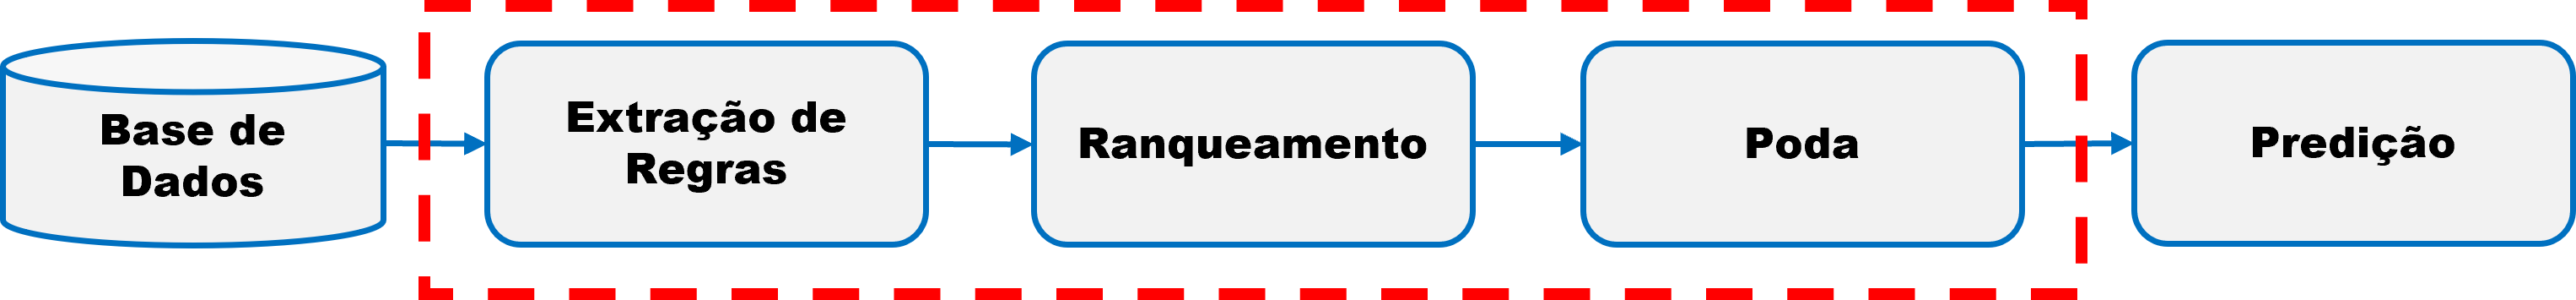
\includegraphics[width=\linewidth]{figuras/fluxo-geral.png}
    \caption{Fluxo geral de indução e predição de um classificador associativo.}
    \label{fig:fluxo_cba}
\end{figure}

No contexto desta dissertação, a seleção de atributos é realizada antes da indução do classificador associativo. Dessa forma, a redução do conjunto de atributos pode alterar os itens disponíveis para a geração de RACs e, consequentemente, influenciar tanto o desempenho preditivo quanto a quantidade e a estrutura das regras produzidas. Esses efeitos motivam a avaliação conjunta do desempenho e da complexidade dos classificadores obtidos após a aplicação do EFS4AC.

%%%%%%%%%%%

%%%%%%%%%%%
\section{Seleção de Atributos}\label{sec:fs} 

A seleção de atributos (\textit{feature selection} (FS))\footnote{Este trabalho utilizará os termos em português e inglês indistintamente.} é uma técnica de pré-processamento amplamente utilizada em aprendizado de máquina (AM), particularmente em conjuntos de dados de alta dimensionalidade \cite{Dhal2022,10.1007/978-3-031-23092-9_12,BARBIERI2024123667}. Seu objetivo consiste em identificar um subconjunto de atributos relevantes a partir do conjunto original, buscando, quando possível, reduzir a redundância entre eles, preservar ou melhorar o desempenho preditivo e reduzir a complexidade dos modelos \cite{Theng2024,Emmoh2024}.

No contexto da classificação associativa, conforme discutido na Seção~\ref{sec:ca}, a redução do número de atributos pode contribuir para diminuir o espaço de busca de regras e a complexidade dos classificadores induzidos. Dessa forma, a aplicação de métodos de FS pode proporcionar diferentes benefícios, entre os quais se destacam:
%%%%%%%%%%%%%%%%%%%%%%%%
\begin{itemize}
    \item \textbf{redução da complexidade e do custo computacional}: a diminuição do número de atributos pode reduzir o espaço de busca e o tempo de treinamento dos algoritmos \cite{Theng2024};

    \item \textbf{melhoria do desempenho e redução do risco de \textit{overfitting}}: a remoção de atributos ruidosos ou irrelevantes pode favorecer a capacidade de generalização dos modelos \cite{Dhal2022};

    \item \textbf{aumento da interpretabilidade e apoio à descoberta de conhecimento}: a utilização de um subconjunto menor de atributos pode facilitar a compreensão dos modelos e a identificação de características relevantes para o problema \cite{Dhal2022,KHAIRE20221060}.
\end{itemize}
%%%%%%%%%%%%%%%%%%%%%%%%

Três são as principais abordagens existentes para realização de FS, a saber \cite{Tan2020,Theng2024}: \textbf{filtro}, \textbf{\textit{embedded}} e \textbf{\textit{wrapper}}. A escolha da abordagem de FS é um ponto crítico, pois ela influencia diretamente a estabilidade do subconjunto de atributos selecionados e o desempenho final do modelo \cite{KHAIRE20221060,BARBIERI2024123667}. Em geral tem-se que:
\begin{itemize}
    \item \textbf{filtro}: constitui a abordagem mais simples e computacionalmente eficiente para a seleção de atributos. Os métodos existentes são independentes do algoritmo de AM que será utilizado \cite{Dhal2022,10.1007/978-3-031-23092-9_12,Theng2024,EBRAHIMIWARKIANI2025129372};
    
    \item \textbf{\textit{wrapper}}: utiliza um algoritmo de AM como mecanismo de avaliação de diferentes subconjuntos de atributos, sendo, portanto, dependente de um algoritmo base. Essa abordagem envolve a indução de múltiplos modelos, o que a torna mais custosa computacionalmente \cite{Theng2024};
    
    \item \textbf{\textit{embedded}}: realiza a seleção de atributos durante o processo de indução do modelo, sendo também dependente do algoritmo utilizado \cite{bashir2022novel,Theng2024}. Nessa abordagem, a relevância dos atributos é incorporada ao mecanismo de treinamento do modelo, como ocorre em árvores de decisão, métodos baseados em regularização e \textit{ensembles} de árvores. Em geral, métodos \textit{embedded} apresentam menor custo computacional que abordagens \textit{wrapper}, pois a seleção é integrada ao treinamento do modelo, embora os subconjuntos obtidos tendam a ser mais dependentes do algoritmo empregado.
\end{itemize}

Neste trabalho, são utilizados métodos de filtro como componentes do EFS4AC, devido à sua independência em relação ao algoritmo de classificação e à sua eficiência computacional. Esses métodos avaliam a relevância dos atributos por meio de critérios estatísticos, informacionais ou de dependência, sem utilizar diretamente o desempenho do classificador como função de avaliação \cite{SolorioFernandez2020,Bouchlaghem2022,Theng2024}.

Em abordagens baseadas em \textit{ranking}, os atributos recebem pontuações ou posições de acordo com o critério adotado. A partir dessa ordenação, um subconjunto pode ser definido mediante um limiar (\textit{threshold}) ou pela seleção de um número predefinido de atributos \cite{geng2007feature,jovic2015review,Theng2024}. Entretanto, a definição do subconjunto final constitui uma decisão adicional, uma vez que o \textit{ranking}, isoladamente, não determina quantos atributos devem ser selecionados.

Os métodos de filtro podem ser classificados em \textbf{univariados} e \textbf{multivariados} \cite{SolorioFernandez2020,Theng2024}. Os métodos univariados avaliam cada atributo individualmente, sem considerar explicitamente suas relações com os demais atributos. Já os métodos multivariados consideram relações entre atributos durante o processo de seleção, podendo incorporar critérios de redundância, dependência e interação \cite{SolorioFernandez2020,Dhal2022,Theng2024}.

Entre as principais vantagens dos métodos de filtro destacam-se a eficiência computacional e a independência em relação ao algoritmo de classificação, características que favorecem sua utilização em diferentes conjuntos de dados e modelos preditivos \cite{Dhal2022,Theng2024}. Por outro lado, os métodos univariados apresentam limitações na identificação de redundâncias e interações entre atributos, enquanto os métodos multivariados podem apresentar maior custo computacional. Além disso, diferentes critérios de avaliação podem produzir ordenações distintas dos atributos, e a escolha do ponto de corte pode influenciar a qualidade do subconjunto selecionado \cite{KHAIRE20221060,Theng2024}. Essa diversidade de critérios e resultados constitui uma das motivações para a combinação de diferentes métodos de seleção de atributos, conforme discutido na próxima subseção.

%%%%%%%%%%%%%%%%%%%%%
\subsection{\textit{Ensemble Feature Selection}}
\label{subsec:efs}

O \textit{Ensemble Feature Selection} (EFS) estende o princípio de aprendizado por \textit{ensemble} ao problema de seleção de atributos, combinando os resultados produzidos por múltiplos seletores-base para obter uma avaliação conjunta da relevância dos atributos \cite{bolon2019ensembles,salman2026review}. A motivação para o uso de EFS decorre do fato de que diferentes métodos de FS podem avaliar os atributos segundo critérios distintos e, consequentemente, produzir diferentes \textit{rankings} ou subconjuntos de atributos. Assim, em vez de depender exclusivamente do resultado de um único seletor, um \textit{ensemble} combina múltiplas avaliações com o objetivo de obter uma solução consensual e reduzir a variabilidade do processo de seleção, favorecendo maior robustez e estabilidade \cite{bolon2019ensembles,salman2026review}.

Diferentemente das abordagens filtro, \textit{wrapper} e \textit{embedded}, que caracterizam a forma como os atributos são avaliados e selecionados, o EFS constitui uma estratégia de combinação de múltiplos métodos de FS. Dessa forma, um EFS pode ser composto por seletores pertencentes a uma mesma abordagem ou a diferentes abordagens, combinando, por exemplo, métodos filtro, \textit{wrapper} e \textit{embedded}.

A diversidade entre os componentes de um EFS pode ser introduzida, principalmente, por meio de duas estratégias \cite{bolon2019ensembles}. Nos \textit{ensembles} homogêneos, um mesmo método de FS é aplicado sob diferentes condições, como diferentes amostras do conjunto de treinamento ou configurações do método, produzindo resultados que são posteriormente combinados. Nos \textit{ensembles} heterogêneos, por sua vez, diferentes métodos de FS são aplicados sobre o mesmo conjunto de dados, permitindo que critérios distintos de avaliação dos atributos contribuam para o resultado final. A Figura~\ref{fig:efs_homogeneo_heterogeneo} ilustra essas duas estratégias. Na Figura~\ref{fig:efs_homogeneo_heterogeneo}, $R_1,\ldots,R_k$ representam os \textit{rankings} produzidos pelo mesmo seletor sob diferentes condições no EFS homogêneo, enquanto $R_1,\ldots,R_m$ representam os \textit{rankings} obtidos por diferentes seletores no EFS heterogêneo. Em ambos os casos, os resultados individuais são encaminhados a uma estratégia de agregação, responsável por produzir uma representação consensual da importância dos atributos.

%%%%%%%%%%%%%%
\begin{figure}[htb]
    \centering
    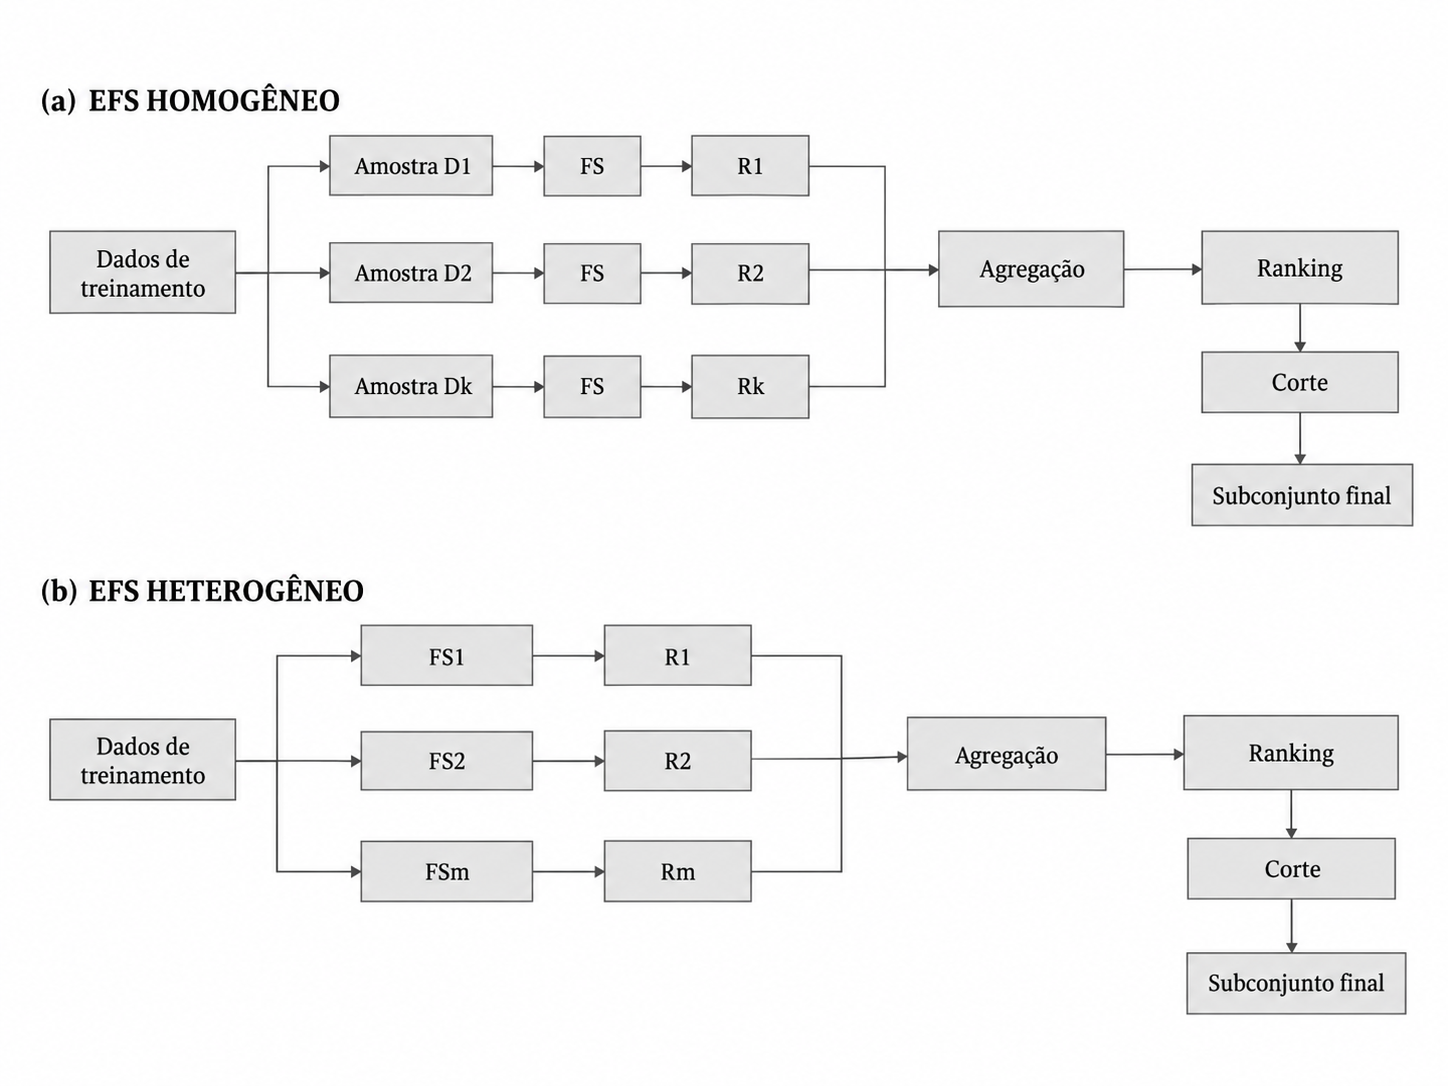
\includegraphics[width=\textwidth]
    {figuras/efs_homogeneo_heterogeneo.png}
    \caption{Estruturas gerais de \textit{Ensemble Feature Selection} homogêneo e heterogêneo. Elaborado pelo autor com base em \citeonline{bolon2019ensembles}.}
    \label{fig:efs_homogeneo_heterogeneo}
\end{figure}
%%%%%%%%%%%%%%

A forma de agregação depende do tipo de saída fornecida pelos seletores-base. Quando os métodos produzem subconjuntos de atributos, esses resultados podem ser combinados diretamente por estratégias de consenso. Quando produzem rankings ou pontuações (scores), diferentes métodos de agregação podem ser utilizados para gerar uma avaliação global da importância dos atributos \cite{bolon2019ensembles}. Nesse segundo caso, torna-se necessária uma etapa adicional de definição do subconjunto final (\textit{thresholding}), responsável por converter a avaliação agregada em um conjunto de atributos selecionados.

Assim, a construção de um EFS envolve diferentes decisões metodológicas, incluindo a composição do conjunto de seletores, a geração de diversidade entre seus componentes, a estratégia de agregação dos resultados individuais e o critério empregado para determinar o subconjunto final de atributos. Essas decisões podem influenciar propriedades importantes do processo de seleção, como estabilidade, robustez e dimensionalidade do subconjunto obtido, bem como o desempenho dos modelos induzidos.

%%%%%%%%%%%

%%%%%%%%%%%
%%%%%%%%%%%%%%%%%%%%%%%%%%%
\section{Critérios de Avaliação}
\label{met_avaliacao}
%%%%%%%%%%%%%%%%%%%%%%%%%%%
%%%teria mais o custo computacional

A avaliação de uma estratégia de seleção de atributos aplicada à classificação não deve considerar apenas o desempenho preditivo do modelo resultante. No contexto deste trabalho, a análise envolve diferentes dimensões, incluindo a capacidade classificatória, a redução da dimensionalidade, a estabilidade do processo de seleção e a complexidade do classificador associativo obtido. Esses critérios permitem avaliar não apenas se a seleção preserva ou melhora a capacidade de predição, mas também seus efeitos sobre o subconjunto de atributos e a estrutura do modelo baseado em regras.

O desempenho preditivo deve ser avaliado sobre dados não utilizados durante o treinamento, permitindo estimar a capacidade de generalização do classificador. Entre as medidas comumente utilizadas estão precisão, revocação e medida-F, que, em problemas multiclasse, podem ser agregadas por estratégias como micro, macro e macro ponderada. Neste trabalho, destaca-se a medida F1-macro, que atribui o mesmo peso a cada classe no cálculo da média dos valores de F1. Para obter estimativas mais confiáveis, podem ser empregados protocolos como \textit{holdout} e validação cruzada (\textit{cross-validation}), incluindo sua versão estratificada. Uma discussão detalhada dessas medidas e estratégias pode ser encontrada em \citeonline{Tan2020}.

No contexto de seleção de atributos, outra dimensão relevante corresponde à redução da dimensionalidade. Seja $F$ o conjunto original de atributos e $S \subseteq F$ o subconjunto selecionado, o percentual de redução pode ser expresso conforme a Equação~\ref{eq:red-fs}. Essa medida permite verificar o quanto uma estratégia de FS reduz o espaço original de atributos. No caso da classificação associativa, essa redução pode produzir efeitos adicionais, uma vez que os atributos selecionados determinam os itens disponíveis para a mineração e, consequentemente, podem modificar o número de \textit{itemsets} e as regras produzidas.

%%%%%%%
\begin{equation}\label{eq:red-fs}
    \text{Redu\c{c}\~{a}o(\%)} =
    \left(
    1 - \frac{|S|}{|F|}
    \right) \times 100
\end{equation}
%%%%%%%

Outro aspecto relevante para métodos de FS e EFS é a estabilidade da seleção. A estabilidade refere-se à capacidade de um método produzir subconjuntos semelhantes quando pequenas alterações são realizadas nos dados de treinamento. Uma estratégia de seleção pode apresentar desempenho preditivo semelhante entre diferentes execuções e, ainda assim, selecionar atributos substancialmente distintos. Em EFS, essa propriedade é particularmente relevante, uma vez que a combinação de múltiplos seletores pode contribuir para reduzir a variabilidade associada às decisões individuais de seleção. A estabilidade pode ser avaliada por meio de medidas que quantificam a similaridade entre os subconjuntos de atributos obtidos em diferentes execuções do processo de seleção.

Em algoritmos baseados em regras, a avaliação pode considerar também propriedades relacionadas à complexidade e à interpretabilidade do modelo. Embora modelos baseados em regras sejam frequentemente considerados inerentemente interpretáveis, a utilização de regras não garante, por si só, uma representação simples \cite{Rudin2019,margot2021interpretability,molnar2022}. Um classificador pode conter um grande número de regras ou regras extensas, tornando sua inspeção difícil. Por esse motivo, propriedades estruturais do modelo são frequentemente utilizadas como aproximações da complexidade interpretativa.

No contexto da classificação associativa, a quantidade de regras é uma dessas medidas e tem sido empregada em diferentes trabalhos \cite{Agnol:2024,math11183978,momac,app12189055,Building2020,DBLP:journals/access/Rajab19,DBLP:conf/kdd/LakkarajuBL16}. Entretanto, o número de regras não deve ser interpretado isoladamente como uma medida completa de interpretabilidade, pois outras propriedades, como o comprimento dos antecedentes e a redundância entre regras, também podem influenciar a complexidade do modelo.

Dessa forma, a avaliação das estratégias investigadas neste trabalho considera diferentes perspectivas complementares. O desempenho preditivo indica a capacidade de generalização do classificador; a redução dimensional caracteriza a capacidade do método de FS em restringir o espaço de atributos; a estabilidade avalia a consistência da seleção diante de perturbações nos dados; e as propriedades estruturais do classificador associativo permitem analisar os efeitos da seleção sobre a complexidade do modelo baseado em regras.

%%%%%%%%%%%
% ==================================================================================================================================

%%%%%%%%%%%%%%%%%%%%%%%%%%%
\chapter{Trabalhos Relacionados}
\label{trabRelac}
%%%%%%%%%%%%%%%%%%%%%%%%%%%

Este capítulo apresenta os trabalhos relacionados às duas vertentes que fundamentam esta pesquisa. A primeira, apresentada na Seção~\ref{sec:fs-ca}, compreende estudos que investigam a utilização de métodos de seleção de atributos em classificadores associativos. A segunda, apresentada na Seção~\ref{ensambleFS}, aborda estratégias de \textit{Ensemble Feature Selection} (EFS), com ênfase na diversidade entre seletores, nos mecanismos de agregação, na estabilidade da seleção e na definição dos subconjuntos finais de atributos. Por fim, a Seção~\ref{sec:consideracoes-relacionados} sintetiza as evidências identificadas e as lacunas que motivam esta pesquisa.

% =====================================================================
% =====================================================================
% =====================================================================
% =====================================================================
\section{Seleção de Atributos em Classificadores Associativos}
\label{sec:fs-ca}
% =====================================================================

A literatura apresenta diferentes estratégias para integrar a seleção de atributos à classificação associativa, que podem ser organizadas em duas categorias principais: seleção externa e seleção interna. Na seleção externa, os atributos são selecionados previamente à construção do classificador associativo, por meio de métodos individuais, híbridos ou baseados em \textit{ensemble} \cite{abubacker2017integrated,alagukumar2025impacts,alazaidah2021feature,alhawari2021classification,ashi2021enhancing,cicek2021assessment,ghareb2018enhanced,piri2019exploring,rad2024framework,sowan2023hybrid}. Na seleção interna, critérios de relevância dos atributos são incorporados à própria construção do classificador, como na seleção de condições durante a geração de regras ou na ponderação de \textit{itemsets} \cite{nandhini2022performance,wu2024novel}.

Esta seção apresenta e analisa trabalhos que combinam seleção de atributos e classificação associativa, destacando as estratégias de integração, os métodos empregados e os principais resultados obtidos. Os trabalhos foram identificados por meio de buscas em bases bibliográficas (\textit{Scopus}, \textit{IEEE Xplore}, \textit{ACM Digital Library}, \textit{Web of Science} e \textit{Google Scholar}), utilizando combinações de termos relacionados à classificação associativa e à seleção de atributos\footnote{A busca utilizou variações da seguinte expressão, adaptadas à sintaxe de cada base consultada: \textit{((``association classification'' OR ``associative classification'' OR ``associative rule mining'' OR ``associative classifier'' OR ``associative classifiers'' OR ``predictive association rules'' OR ``predictive association rule'' OR ``class association rules'' OR ``class association rule'' OR ``classification association rules'' OR ``classification association rule'') AND (``feature selection'' OR ``attribute selection'' OR ``feature ranking'' OR ``item selection''))}. Nas bases que permitiam a delimitação dos campos de busca, a consulta foi aplicada ao título, resumo e palavras-chave, utilizando, por exemplo, o operador \texttt{TITLE-ABS-KEY} na Scopus.}. A seleção priorizou estudos que investigam explicitamente a utilização de métodos de seleção de atributos em classificadores associativos, considerando diferentes estratégias de integração. Ao todo, foram selecionados 12 trabalhos para análise.

% ---------------------------------------------------------------------
\subsection{Visão Geral dos Trabalhos}
\label{subsec:trabalhos-ca}
% ---------------------------------------------------------------------

Os trabalhos analisados são apresentados conforme a forma de integração da seleção de atributos à classificação associativa. Inicialmente, são discutidas as abordagens de seleção externa, seguidas pelas estratégias que incorporam critérios de relevância à construção do classificador. Por fim, destaca-se uma proposta de \textit{Ensemble Feature Selection} particularmente relacionada a esta dissertação.

%ref
\citeonline{alazaidah2021feature} comparam nove métodos de seleção de atributos (ABB-IEP, ABB-LIU, Focus, LVF, Relief, SBS-LIU, SBS-IEP, SFS-IEP e SFS-LIU) aplicados como pré-processamento de cinco classificadores associativos (CBA, CBA2, CFAR, CMAR e CPAR). A avaliação considera conjuntos de dados com diferentes tipos de atributos e indica que não há um método de seleção consistentemente superior: ABB-IEP e ABB-LIU destacam-se em conjuntos com atributos nominais, enquanto Relief apresenta melhores resultados em conjuntos com atributos numéricos. O estudo evidencia, assim, que a eficácia da seleção depende das características dos dados e do classificador associativo utilizado.

%ref
\citeonline{ghareb2018enhanced} propõem três métodos de seleção de atributos baseados em filtros (CRFM, MCDM e OR2) para categorização de textos em língua árabe. Os métodos são comparados com doze estratégias tradicionais de seleção, utilizando três conjuntos de documentos e os classificadores Naive Bayes e classificação associativa baseada em Apriori. Os resultados mostram que, na classificação associativa, MCDM e OR2 apresentam os melhores desempenhos em diferentes conjuntos de dados, enquanto a quantidade de regras geradas também varia conforme o filtro utilizado. O estudo evidencia, assim, que a escolha do método de seleção influencia tanto o desempenho preditivo quanto a estrutura do classificador associativo.

%ref
\citeonline{alhawari2021classification} investigam a seleção de atributos na classificação de avaliações textuais de aplicativos relacionadas à manutenção de software. Após o processamento dos textos, os autores aplicam os filtros \textit{Information Gain} (IG) e $\chi^2$ como pré-processamento de classificadores tradicionais e associativos (CBA, CBA2, CMAR e CPAR). O trabalho também propõe o ACRM (\textit{Associative Classification for Reviews Mining}), que utiliza FP-Growth para mineração de padrões e os critérios de confiança e \textit{conviction} para classificação. Os resultados indicam melhorias no desempenho após a seleção de atributos, com IG apresentando, em geral, melhores resultados que $\chi^2$, embora os ganhos sejam menores nos classificadores associativos.

%ref
\citeonline{ashi2021enhancing} investigam o efeito da seleção de atributos na predição de evasão de clientes (\textit{customer churn}) utilizando os classificadores associativos CBA, CBA2, CPAR e FARC-HD. Os autores empregam o método \textit{Sequential Backward Search using Inconsistent Examples Pairs} (SBS-IEP) como etapa de pré-processamento e comparam os classificadores com e sem seleção de atributos. Os resultados mostram uma redução na quantidade de regras geradas pelos quatro classificadores, embora em proporções distintas, evidenciando que a seleção de atributos também pode contribuir para a redução da complexidade dos modelos associativos.

%ref
\citeonline{piri2019exploring} investigam a seleção de atributos na classificação associativa de dados de cardiotocografia para determinação do estado fetal. Após a discretização dos atributos contínuos por um método baseado em entropia, os autores utilizam o \textit{ExtraTreesClassifier} para obter um \textit{ranking} de importância, selecionando os dez atributos mais relevantes para o classificador CBA. Os experimentos consideram as variantes CBA-M1 e CBA-M2, com e sem poda. Na configuração CBA-M1 com poda, a seleção eleva a acurácia de 83\% para 84\% e reduz a quantidade de regras de 48 para 2. Os resultados evidenciam que a seleção de atributos pode contribuir para reduzir significativamente a complexidade do modelo associativo, mesmo quando os ganhos preditivos são modestos.

%ref
\citeonline{cicek2021assessment} investigam a classificação associativa de dados de expressão gênica para distinguir indivíduos positivos e negativos para COVID-19. O conjunto de dados contém 15.979 genes e 234 amostras, caracterizando um problema de alta dimensionalidade. Os autores utilizam LASSO como etapa de pré-processamento, reduzindo o conjunto de 15.979 para 31 genes, posteriormente utilizados pelo classificador associativo CBA. As regras de associação de classe geradas permitem identificar combinações de genes associadas às classes, contribuindo para a interpretação dos resultados. Entretanto, o estudo não apresenta uma comparação experimental do classificador com e sem seleção de atributos.

%ref
\citeonline{alagukumar2025impacts} investigam a combinação de seleção de atributos e discretização na classificação associativa de dados de expressão gênica. Os autores avaliam três filtros baseados em informação mútua (JIM, JMI e JMI3), combinados com cinco métodos supervisionados de discretização (MDLP, CAIM, CACC, AMEVA e Chi-Merge). Os atributos selecionados são discretizados e utilizados pelos classificadores associativos CBA e CMAR. A avaliação considera tanto o desempenho preditivo quanto o número de intervalos e \textit{itemsets}, permitindo analisar os efeitos das diferentes combinações de pré-processamento sobre a representação dos dados e a classificação.

%ref
Além das abordagens que utilizam a seleção de atributos como pré-processamento de classificadores associativos convencionais, alguns estudos propõem arquiteturas híbridas ou incorporam mecanismos de seleção à própria construção dos modelos. \citeonline{abubacker2017integrated} propõem uma arquitetura híbrida para classificação de mamografias que combina seleção de atributos, mineração de regras de associação de classe (RACs) e classificadores neurais. A seleção utiliza \textit{Correlation-based Feature Selection} (CFS) associado a uma busca genética, enquanto a mineração emprega uma versão modificada do \textit{Genetic Association Rule Mining} (GARM). As RACs geradas são utilizadas como entrada dos classificadores ACNN e ACFNN, baseados, respectivamente, em redes neurais e redes neuro-fuzzy. Diferentemente dos classificadores associativos convencionais, a arquitetura utiliza as regras como entrada para modelos neurais, caracterizando uma abordagem híbrida.

%ref
Diferentemente das abordagens que realizam seleção de atributos como pré-processamento, \citeonline{nandhini2022performance} investigam critérios de seleção incorporados à geração de regras do classificador associativo CPAR. Os autores substituem o critério original \textit{FOIL's Information Gain} por \textit{Gain Ratio} (GR) e \textit{Mutual Information Gain} (IG), originando as variantes CPAR-GR e CPAR-IG. Também avaliam as medidas \textit{Laplace Accuracy} e \textit{Likelihood Ratio} para avaliação e seleção das regras. Os resultados em conjuntos de dados médicos indicam desempenho favorável do CPAR-GR em relação ao CPAR original, embora sem superioridade consistente em todas as configurações. O estudo demonstra, assim, que a escolha do critério de seleção durante a geração das regras pode influenciar o desempenho preditivo do classificador.

%ref
\citeonline{wu2024novel} propõem o MCWCAR (\textit{Mutual Information and Correlation Coefficient Weighted Class Association Rule Mining}) para predição de defeitos de software. Diferentemente das abordagens que selecionam previamente um subconjunto de atributos, o método incorpora critérios de relevância à própria mineração de \textit{itemsets}. A informação mútua é utilizada para ponderar atributos na mineração de \textit{itemsets} sem classe, enquanto coeficientes de correlação atribuem pesos aos itens associados às classes com e sem defeito. Essas ponderações influenciam a seleção dos \textit{itemsets} frequentes que dão origem às regras de associação de classe, caracterizando uma abordagem de seleção de atributos interna ao processo de classificação associativa, sem a geração prévia de um subconjunto global de atributos. Os resultados experimentais indicam desempenho superior ao dos classificadores CWCAR, CBA3 e ACAR nas métricas \textit{Balance}, MCC e G-Mean, com diferenças estatisticamente significativas nas comparações realizadas.

%ref
\citeonline{rad2024framework} propõem um \textit{framework} para detecção de moedas falsificadas baseado em classificação associativa fuzzy. A proposta introduz o PFA (\textit{Pruned Fuzzy Associative Classifier}) e o mecanismo Engine\_FAFS, que utiliza regras de associação fuzzy para selecionar atributos presentes nos antecedentes das regras consideradas relevantes. Diferentemente das abordagens que empregam filtros tradicionais, a seleção é realizada a partir das próprias regras de associação, sendo posteriormente integrada à construção do classificador associativo PFA, que utiliza regras com consequentes de classe. O \textit{framework} também incorpora poda de regras baseada em dependência estatística e otimização por \textit{Particle Swarm Optimization} (PSO), incluindo o ajuste do parâmetro $\delta$, responsável por controlar o tamanho do subconjunto selecionado.

%ref
Por fim, destaca-se uma proposta que, diferentemente das estratégias individuais de seleção ou dos mecanismos incorporados à geração de regras, combina múltiplos seletores de atributos antes da construção do classificador associativo. \citeonline{sowan2023hybrid} propõem duas estratégias de seleção de atributos para classificação associativa de câncer de mama. A primeira, denominada WARF (\textit{Weighted Average of Relative Frequency}), combina os filtros CFS, \textit{Information Gain}, \textit{Gain Ratio}, $\chi^2$ e ReliefF em um \textit{ensemble}, utilizando \textit{rankings} de importância e frequências relativas de seleção dos atributos para identificar um subconjunto relevante, posteriormente utilizado pelo classificador associativo PCBA. A segunda estratégia, Hybrid PSO-WARF, incorpora uma busca baseada em \textit{Particle Swarm Optimization} (PSO) e na avaliação de subconjuntos por classificadores, constituindo uma abordagem híbrida entre filtro e \textit{wrapper}. Os resultados experimentais indicam melhorias no desempenho preditivo em comparação com diferentes métodos individuais e classificadores associativos de referência. Entre os estudos analisados, este é o mais diretamente relacionado à presente dissertação, por combinar múltiplos seletores de atributos com classificação associativa. Entretanto, sua estratégia de agregação baseia-se em frequências relativas e médias ponderadas de importância, diferentemente dos métodos de agregação de \textit{rankings} investigados nesta dissertação.

% ---------------------------------------------------------------------
\subsection{Síntese Comparativa dos Trabalhos} \label{subsec:sintese-ca}
% ---------------------------------------------------------------------

A análise dos trabalhos apresentados na Seção~\ref{subsec:trabalhos-ca} evidencia diferentes formas de integração da seleção de atributos à classificação associativa, distinguindo abordagens de seleção externa e interna. A Tabela~\ref{tab:sintese-ca} sintetiza os 12 estudos quanto ao tipo de integração, aos métodos de seleção de atributos, às estratégias de utilização, aos classificadores associativos empregados e às avaliações e comparações realizadas. Os trabalhos são apresentados na mesma ordem da subseção anterior, facilitando a correspondência entre suas descrições e a análise comparativa. A partir dessa síntese, são discutidos os principais aspectos metodológicos que diferenciam os estudos, permitindo identificar tendências, limitações e oportunidades de investigação.

%%%%%%%%%%%%%%%%%%%%%%%%%%
%%%%%%%%%%%%%%%%%%%%%%%%%%
\begingroup
\scriptsize
\setlength{\tabcolsep}{3pt}
\renewcommand{\arraystretch}{1.25}

\begin{longtable}{|
p{2.15cm}|
p{1.25cm}|
p{2.65cm}|
p{3.05cm}|
p{1.95cm}|
p{3.55cm}|}

\caption{Síntese comparativa dos trabalhos que integram seleção de atributos e classificação associativa.}
\label{tab:sintese-ca}\\

\hline
\textbf{Referência} &
\textbf{Tipo} &
\textbf{Método de FS} &
\textbf{Estratégia de uso} &
\textbf{CA} &
\textbf{Avaliação/Comparação} \\
\hline
\endfirsthead

\multicolumn{6}{c}{\tablename\ \thetable{} -- continuação}\\
\hline
\textbf{Referência} &
\textbf{Tipo} &
\textbf{Método de FS} &
\textbf{Estratégia de uso} &
\textbf{CA} &
\textbf{Avaliação/Comparação} \\
\hline
\endhead

\hline
\multicolumn{6}{r}{\textit{continua na próxima página}}\\
\endfoot

\hline
\endlastfoot

\citeonline{alazaidah2021feature} &
Externa &
ABB-IEP, ABB-LIU, Focus, LVF, Relief, SBS-LIU, SBS-IEP, SFS-IEP e SFS-LIU &
Comparação de nove métodos de FS, aplicados individualmente como pré-processamento &
CBA, CBA2, CFAR, CMAR e CPAR &
Compara os métodos de FS em diferentes conjuntos de dados e classificadores associativos \\
\hline

\citeonline{ghareb2018enhanced} &
Externa &
CRFM, MCDM, OR2 e doze métodos tradicionais &
Proposição de três filtros e comparação individual com métodos de referência &
CA baseada em Apriori &
Compara o desempenho dos seletores e seus efeitos sobre a quantidade de regras \\
\hline

\citeonline{alhawari2021classification} &
Externa &
IG e $\chi^2$ &
Comparação de dois filtros aplicados separadamente como pré-processamento &
CBA, CBA2, CMAR, CPAR e ACRM &
Compara classificadores tradicionais e associativos após a seleção de atributos \\
\hline

\citeonline{ashi2021enhancing} &
Externa &
SBS-IEP &
Método individual de seleção sequencial aplicado antes da classificação &
CBA, CBA2, CPAR e FARC-HD &
Compara os classificadores com e sem FS, incluindo a quantidade de regras \\
\hline

\citeonline{piri2019exploring} &
Externa &
ExtraTreesClassifier &
Método individual baseado em \textit{ranking} de importância, com seleção dos dez primeiros atributos &
CBA &
Compara CBA-M1 e CBA-M2, com e sem poda e seleção de atributos \\
\hline

\citeonline{cicek2021assessment} &
Externa &
LASSO &
Método individual para redução de dimensionalidade antes da classificação &
CBA &
Avalia o classificador com atributos selecionados, sem comparação com o conjunto completo \\
\hline

\citeonline{alagukumar2025impacts} &
Externa &
JIM, JMI e JMI3 &
Comparação de filtros individuais combinados experimentalmente com métodos de discretização &
CBA e CMAR &
Compara combinações de FS e discretização quanto ao desempenho, intervalos e \textit{itemsets} \\
\hline

\citeonline{abubacker2017integrated} &
Externa &
CFS com busca genética &
Seleção prévia integrada a uma arquitetura híbrida que utiliza RACs como entrada de modelos neurais &
GARM + ACNN/ACFNN &
Avalia o desempenho da arquitetura híbrida em dados de mamografia \\
\hline

\citeonline{nandhini2022performance} &
Interna &
FOIL-IG, GR e IG &
Critérios alternativos de seleção de condições durante a geração das regras &
CPAR, CPAR-GR e CPAR-IG &
Compara variantes do CPAR e medidas de avaliação e seleção de regras \\
\hline

\citeonline{wu2024novel} &
Interna &
Informação mútua e coeficientes de correlação &
Ponderação de atributos e itens incorporada à mineração de \textit{itemsets}, sem seleção prévia de subconjunto global &
MCWCAR &
Compara o desempenho com CWCAR, CBA3 e ACAR \\
\hline

\citeonline{rad2024framework} &
Externa &
Engine\_FAFS &
Seleção de atributos baseada em regras de associação fuzzy, integrada a um \textit{framework} com PSO e poda de regras &
PFA &
Avalia o \textit{framework} proposto para detecção de moedas falsificadas \\
\hline

\citeonline{sowan2023hybrid} &
Externa &
WARF: CFS, IG, GR, $\chi^2$ e ReliefF; Hybrid PSO-WARF &
\textit{Ensemble} de filtros baseado em frequências relativas e médias ponderadas; variante híbrida com PSO &
PCBA &
Compara métodos individuais, estratégias propostas e classificadores associativos de referência \\
\hline

\end{longtable}
\endgroup
%%%%%%%%%%%%%%%%%%%%%%%%%%
%%%%%%%%%%%%%%%%%%%%%%%%%%

%%%%%%%%%%%%%%%%%%%%%%%%%%
\noindent\textbf{Tipo de integração.} Em dez dos 12 estudos analisados, a seleção de atributos ocorre antes da construção do classificador associativo, caracterizando uma abordagem externa. Essa configuração favorece a modularidade, permitindo modificar o método de seleção sem necessariamente alterar o algoritmo de classificação, como observado em \citeonline{alazaidah2021feature} e \citeonline{sowan2023hybrid}.

Em contrapartida, \citeonline{nandhini2022performance} e \citeonline{wu2024novel} incorporam critérios de relevância diretamente à construção do classificador associativo, seja durante a geração das regras, seja na mineração de \textit{itemsets}. Nessas abordagens, a seleção não resulta previamente em um subconjunto global de atributos.

Uma particularidade é apresentada por \citeonline{rad2024framework}, cuja seleção é orientada por regras de associação fuzzy, embora anteceda a construção do classificador associativo final. Assim, o estudo é classificado como seleção externa, mas distingue-se das abordagens tradicionais de pré-processamento.

%%%%%%%%%%%%%%%%%%%%%%%%%%
\noindent\textbf{Métodos de FS.} Os estudos analisados apresentam diversidade nos critérios empregados para avaliar a relevância dos atributos. Medidas baseadas em teoria da informação aparecem de forma recorrente. \citeonline{nandhini2022performance} exploram FOIL-IG, GR e IG no CPAR; \citeonline{alhawari2021classification} utilizam IG e $\chi^2$; \citeonline{alagukumar2025impacts} analisam JIM, JMI e JMI3; e \citeonline{wu2024novel} incorporam informação mútua à ponderação dos atributos. Essa recorrência evidencia a importância das medidas de dependência e relevância na seleção de atributos para classificação associativa.

Entretanto, os resultados não apontam para um critério de seleção consistentemente superior. \citeonline{alazaidah2021feature} identificam comportamentos distintos conforme o tipo dos atributos; \citeonline{ghareb2018enhanced} observam variações entre métodos de seleção e conjuntos de dados; e \citeonline{nandhini2022performance} mostram que a substituição do critério utilizado pelo CPAR influencia o desempenho preditivo, embora sem superioridade consistente em todas as configurações. Em conjunto, esses estudos indicam que diferentes critérios de seleção podem produzir resultados distintos conforme as características dos dados e do classificador associativo.

Também são empregados métodos baseados em modelos e mecanismos de busca. \citeonline{cicek2021assessment} utilizam LASSO em um cenário de elevada dimensionalidade; \citeonline{piri2019exploring} empregam a importância dos atributos calculada pelo \textit{ExtraTreesClassifier}; \citeonline{abubacker2017integrated} combinam CFS com busca genética; e \citeonline{ashi2021enhancing} utilizam busca sequencial para eliminação de atributos. Essas estratégias ampliam a diversidade metodológica observada na literatura.

Entre os estudos analisados, \citeonline{sowan2023hybrid} distinguem-se pela combinação de diferentes critérios de relevância em um \textit{ensemble}, em vez da aplicação isolada dos métodos de seleção. Essa característica aproxima a proposta da presente pesquisa, embora os mecanismos de combinação adotados sejam distintos daqueles investigados no EFS4AC.

%%%%%%%%%%%%%%%%%%%%%%%%%%
\noindent\textbf{Estratégias de uso.} Os estudos apresentam três formas principais de utilização dos métodos de FS: aplicação de um seletor individual, comparação de diferentes seletores utilizados separadamente e combinação de múltiplos métodos para produzir uma seleção consensual. As duas primeiras predominam nos trabalhos analisados, enquanto a terceira é representada por \citeonline{sowan2023hybrid}, que propõem o WARF. Essa distinção evidencia que, embora a comparação entre métodos de FS esteja presente na literatura de classificação associativa, a investigação de estratégias de combinação de seus resultados permanece menos explorada.

%%%%%%%%%%%%%%%%%%%%%%%%%%
\noindent\textbf{Avaliações/Comparações.} Além do desempenho preditivo, alguns estudos consideram os efeitos da seleção de atributos sobre propriedades dos modelos associativos. \citeonline{ashi2021enhancing} e \citeonline{piri2019exploring} avaliam a quantidade de regras geradas, enquanto \citeonline{alagukumar2025impacts} investigam os efeitos conjuntos da seleção e da discretização sobre o número de intervalos e \textit{itemsets}. Essas avaliações evidenciam a importância de considerar aspectos estruturais dos modelos, além de sua capacidade preditiva.

Os estudos também apresentam diferenças quanto aos procedimentos de avaliação experimental. \citeonline{nandhini2022performance} utilizam testes estatísticos para comparar variantes do CPAR; \citeonline{alhawari2021classification} complementam as comparações com testes de significância e medidas de tamanho de efeito; e \citeonline{wu2024novel} empregam Scott-Knott ESD e Wilcoxon \textit{signed-rank}. Por outro lado, alguns trabalhos concentram seus experimentos em aplicações específicas e em conjuntos de dados mais restritos, como \citeonline{abubacker2017integrated}, \citeonline{cicek2021assessment}, \citeonline{piri2019exploring} e \citeonline{rad2024framework}. Essas diferenças metodológicas dificultam a comparação direta dos resultados reportados.

Em conjunto, os estudos evidenciam diferentes possibilidades de aplicação da seleção de atributos à classificação associativa, com resultados dependentes dos métodos e das características dos dados. A combinação de múltiplos seletores constitui uma alternativa ainda pouco explorada nesse contexto, motivando a análise das estratégias de \textit{Ensemble Feature Selection} apresentada na Seção~\ref{ensambleFS}.

%=====================================================================
% 3.2 -- ENSEMBLE FEATURE SELECTION
%=====================================================================
%%%%%%%%%%%%%%%%%%%%%%%%%%%
\section{\textit{Ensemble Feature Selection}}\label{ensambleFS}
%%%%%%%%%%%%%%%%%%%%%%%%%%%

O \textit{Ensemble Feature Selection} (EFS) combina resultados de diferentes métodos de seleção de atributos para reduzir a dependência de um único critério de avaliação e explorar a complementaridade entre os seletores \citeonline{bolon2019ensembles}. Sua construção envolve decisões relacionadas à composição do \textit{ensemble}, à diversidade entre os métodos, à representação e agregação dos resultados e à definição do subconjunto final de atributos. Essas decisões podem influenciar tanto a seleção obtida quanto sua estabilidade e capacidade de generalização, conforme discutido por \citeonline{akhy2024comprehensive}.

Esta seção apresenta e analisa 22 estudos primários sobre EFS, identificados por meio de buscas em bases bibliográficas (\textit{Scopus}, \textit{IEEE Xplore}, \textit{ACM Digital Library}, \textit{Web of Science} e \textit{Google Scholar}), utilizando combinações de termos relacionados a \textit{ensemble feature selection} e agregação de \textit{rankings}\footnote{A expressão de referência utilizada na Scopus foi \textit{TITLE((ensemble* W/2 ``feature selection'') OR (``rank aggregation'' W/2 ``feature selection''))}, com adaptações à sintaxe das demais bases consultadas.}. Trabalhos de revisão foram utilizados como apoio conceitual, mas não integram a comparação metodológica. A Tabela~\ref{tab:efs} sintetiza tais estudos, considerando a composição do \textit{ensemble}, a representação dos resultados, as estratégias de agregação, os critérios adicionais empregados, a definição do subconjunto final e as formas de avaliação. Com base nessa caracterização, as subseções seguintes discutem comparativamente as principais decisões metodológicas identificadas na literatura. Entre os estudos analisados, sete apresentam maior proximidade com as decisões investigadas nesta pesquisa: \citeonline{abasabadi2021automatic}, \citeonline{drotar2019ensemble}, \citeonline{fu2023reranking}, \citeonline{janani2023ensemble}, \citeonline{kaur2023mcdm}, \citeonline{seijopardo2019automatic} e \citeonline{zhang2019ensemble}. Esses trabalhos recebem maior aprofundamento ao longo da discussão, considerando aspectos relacionados à composição do \textit{ensemble}, à agregação dos resultados e à definição do subconjunto final de atributos.

%%%%%%%%%%%%%%%%%%%%%
%%%%%%%%%%%%%%%%%%%%%
\begin{sidewaystable}[p]
\centering
\caption{Síntese dos 22 estudos primários de \textit{Ensemble Feature Selection} analisados.}
\label{tab:efs}
\fontsize{8}{9.2}\selectfont
\setlength{\tabcolsep}{2.5pt}
\renewcommand{\arraystretch}{1.10}
\begin{tabular}{|P{2.3cm}|P{2.6cm}|P{2.3cm}|P{2.8cm}|P{3.0cm}|P{3.0cm}|P{2.6cm}|}
\hline
\textbf{Trabalho} &
\textbf{Composição do \textit{ensemble}} &
\textbf{Representação} &
\textbf{Agregação / consenso} &
\textbf{Diversidade / pesos / critérios adicionais} &
\textbf{Definição do subconjunto} &
\textbf{Avaliação} \\ \hline
\hline
\citeonline{abasabadi2021automatic} & Múltiplos ranqueadores & \textit{Rankings} & \textit{Fast non-dominated sorting} & Múltiplos ranqueadores (geração de diversidade) & Limiar automático & Desempenho e número de atributos \\ \hline
\citeonline{abellana2022ensemble} & Filtros heterogêneos & \textit{Scores}\slash \textit{rankings} & EDAS & Critérios heterogêneos & Retenção de 20\% dos atributos & AUC, redução dimensional e estabilidade \\ \hline
\citeonline{drotar2019ensemble} & Filtros heterogêneos & \textit{Rankings} & Plurality, STV, Borda e Borda ponderada & \textit{Mean-shift clustering} e similaridade entre ranqueadores & Top-$k$/número requerido de atributos & Relevância, estabilidade e classificação \\ \hline
\citeonline{fu2023reranking} & Filtros heterogêneos univariados e multivariados & \textit{Rankings} & TOPSIS e NSGA-III & Complementaridade uni\slash multivariada & Otimização multiobjetivo & Acurácia e F-measure \\ \hline
\citeonline{geng2026stability} & U-test, RFECV, LASSO e informação mútua & Subconjuntos\slash indicadores & Combinação linear ponderada & Pesos otimizados por Bayes e estabilidade entre \textit{folds} & Consenso de seleção e interseção entre \textit{folds} & Desempenho interno/externo e estabilidade \\ \hline
\citeonline{hashemi2021pareto} & Filtros heterogêneos & \textit{Rankings}\slash matriz de decisão & Pareto e ordenação não dominada & Relevância e redundância & Número de atributos definido experimentalmente & Acurácia, F-score e tempo \\ \hline
\citeonline{he2023ensemble} & Filtros heterogêneos & \textit{Rankings}\slash subconjuntos & Combinação ponderada & Pesos adaptativos por \textit{softmax} & Top-$k$ & Desempenho e adequação dos seletores \\ \hline
\citeonline{janani2023ensemble} & Filtros heterogêneos & \textit{Rankings} & IOWA, NWBM, BON-OWA e BON-IOWA & Ponderação por entropia & Top-$k$ & Acurácia, F-measure, precisão e revocação \\ \hline
\citeonline{joseph2025hybrid} & Filtros heterogêneos & \textit{Rankings} & Borda, MC4 e Random Dictator com distância de Kendall & Diversidade entre métodos de agregação & Etapa \textit{wrapper}/RFE & Desempenho preditivo \\ \hline
\citeonline{kaur2023mcdm} & $\chi^2$, correlação, InfoGain e ReliefF & \textit{Scores} & TOPSIS & Critérios heterogêneos & Seleção a partir do \textit{score} final & nMCC e G-measure \\ \hline
\citeonline{kavitha2025decision} & Filtros heterogêneos & \textit{Rankings}\slash matriz de preferência & TOPSIS, VIKOR, CODAS e variantes & Representação qROPHF & \textit{Ranking} seguido de seleção & Desempenho e significância estatística \\ \hline
\end{tabular}
\end{sidewaystable}

\begin{sidewaystable}[p]
\ContinuedFloat
\centering
\caption{Síntese dos 22 estudos primários de \textit{Ensemble Feature Selection} analisados (continuação).}
\fontsize{8}{9.2}\selectfont
\setlength{\tabcolsep}{2.5pt}
\renewcommand{\arraystretch}{1.10}
\begin{tabular}{|P{2.3cm}|P{2.6cm}|P{2.3cm}|P{2.8cm}|P{3.0cm}|P{3.0cm}|P{2.6cm}|}
\hline
\textbf{Trabalho} &
\textbf{Composição do \textit{ensemble}} &
\textbf{Representação} &
\textbf{Agregação / consenso} &
\textbf{Diversidade / pesos / critérios adicionais} &
\textbf{Definição do subconjunto} &
\textbf{Avaliação} \\ \hline
\hline
\citeonline{lin2024ensemble} & SU, FDR e ReliefF com complementaridade discriminante & Subconjuntos & Estratégia de agregação aprimorada & Complementaridade entre critérios & Subconjunto orientado pela capacidade classificatória & Desempenho e redução dimensional \\ \hline
\citeonline{loggenberg2026cross} & 18 métodos de FS baseados em PLS & \textit{Rankings}\slash frequência & \textit{Weighted Borda Count} & Pesos por SRD e desempenho no treinamento & Cotovelo adaptativo e refinamento top-15\% & Transferibilidade, desempenho e redução \\ \hline
\citeonline{ma2024ensemble} & Múltiplos critérios baseados em \textit{neighbourhood rough sets} & \textit{Scores} & Fusão multicritério & Critérios heterogêneos & Busca sequencial & Desempenho preditivo \\ \hline
\citeonline{mera2021framework} & Múltiplos métodos de FS & \textit{Rankings}\slash subconjuntos & Consenso por frequência & Configuração flexível & Limiar de consenso configurável & Desempenho e estabilidade \\ \hline
\citeonline{olabisi2025heterogeneous} & Filtros estatísticos heterogêneos & \textit{Rankings} & Borda & Complementaridade entre filtros & Limiar seguido de consolidação & Desempenho em detecção de \textit{phishing} \\ \hline
\citeonline{seijopardo2019automatic} & Ranqueadores em diferentes configurações & \textit{Rankings} & Desenhos CT e TC com diferentes combinações & Perturbação\slash configuração do \textit{ensemble} & Percentuais fixos ou limiar automático por complexidade & Erro de classificação e número de atributos \\ \hline
\citeonline{chinglensana2026ef} & mRMR, PCFS, JoMIC e MIFS-ND & \textit{Rankings}\slash subconjuntos & Consenso por frequência & Particionamento, refinamento iterativo e controle de redundância & Consenso entre ranqueadores e poda por correlação & Desempenho, redução e robustez \\ \hline
\citeonline{tang2023ensemble} & Filtros heterogêneos & \textit{Scores} & TOPSIS & Ponderação por entropia & \textit{Ranking} seguido de seleção & Desempenho preditivo \\ \hline
\citeonline{wu2023ecm} & Múltiplos seletores & Subconjuntos\slash votos & Coassociação e \textit{Feature Kernel} & Relações entre atributos & Núcleo inicial por coassociação; seleção até atingir $k$ atributos & Desempenho, robustez e estabilidade \\ \hline
\citeonline{zhang2019ensemble} & SAM, InfoGain, GeoDE e ReliefF sob \textit{bootstrap} & \textit{Rankings} & \textit{Rank Products} & Ponderação pela estabilidade & Percentual de atributos & AUC e estabilidade \\ \hline
\citeonline{zheng2019feature} & Tsallis e \textit{Markov blanket} sob múltiplas evidências & Subconjuntos\slash evidências & Dempster--Shafer & Ponderação por evidência & Resultado da fusão & Desempenho preditivo \\ \hline
\end{tabular}
\end{sidewaystable}
%%%%%%%%%%%%%%%%%%%%%
%%%%%%%%%%%%%%%%%%%%%

%%%%%%%%%%%%%%%%%%%%%
%%%%%%%%%%%%%%%%%%%%%
\subsection{Configuração do \textit{Ensemble} e Representação dos Resultados}
\label{subsec:efs-configuracao}

Uma das primeiras decisões na construção de um EFS refere-se à composição do \textit{ensemble} e à forma de introduzir diversidade entre os seletores. Em configurações heterogêneas, diferentes métodos de seleção de atributos são aplicados ao mesmo conjunto de treinamento, explorando critérios distintos de relevância, dependência ou redundância. Essa estratégia é adotada por \citeonline{drotar2019ensemble}, \citeonline{abellana2022ensemble}, \citeonline{kaur2023mcdm}, \citeonline{janani2023ensemble}, \citeonline{lin2024ensemble}, \citeonline{he2023ensemble} e \citeonline{joseph2025hybrid}, entre outros. A combinação de métodos com diferentes critérios busca explorar informações complementares e reduzir a dependência de um único seletor.

Entre os trabalhos que exploram essa configuração, \citeonline{drotar2019ensemble} combinam oito métodos de filtro e investigam a diversidade entre os resultados produzidos. Os autores propõem o agrupamento dos ranqueadores por meio do algoritmo \textit{mean-shift}, representando cada grupo por um \textit{ranking} médio antes da agregação. Essa estratégia busca reduzir a influência de seletores que apresentam resultados semelhantes, evitando que métodos redundantes tenham participação excessiva na formação do consenso. De forma relacionada, \citeonline{abasabadi2021automatic} propõem o \textit{Automatic Thresholding Feature Selection} (ATFS), que combina métodos de filtro e considera a similaridade entre os \textit{rankings} por meio de medidas de correlação, incluindo Spearman e Kendall. Embora empreguem mecanismos distintos, ambos os trabalhos destacam a importância de considerar a relação entre os seletores, e não apenas a quantidade de métodos combinados.

Outras configurações heterogêneas são investigadas por \citeonline{fu2023reranking} e \citeonline{janani2023ensemble}. Os primeiros combinam seis métodos de filtro, incluindo Chi-quadrado, Gini, Fisher Score, ReliefF, mRMR e CMIM, abrangendo diferentes critérios de avaliação dos atributos. Já \citeonline{janani2023ensemble} utilizam cinco métodos de seleção, incluindo abordagens baseadas em relevância e redundância, para investigar diferentes operadores de agregação. Em ambos os casos, a utilização de seletores heterogêneos permite reunir diferentes perspectivas sobre a importância dos atributos, embora o tratamento dessas informações na etapa de agregação seja distinto.

A diversidade também pode ser introduzida por meio de perturbações nos dados de treinamento. Essa estratégia é explorada por \citeonline{zhang2019ensemble}, que propõem o \textit{Ensemble Feature Selection Integrating Stability} (EFSIS). O método combina diferentes funções de seleção com amostras geradas por \textit{bootstrap}, permitindo avaliar tanto a relevância dos atributos quanto a consistência dos resultados diante de variações nos dados. Diferentemente das abordagens que exploram apenas a heterogeneidade dos seletores, o EFSIS incorpora a estabilidade como um componente adicional na construção do \textit{ensemble}.

Além da composição do \textit{ensemble}, a representação dos resultados produzidos pelos métodos de base influencia diretamente as possibilidades de combinação. Os seletores podem fornecer \textit{rankings}, \textit{scores} de relevância ou subconjuntos de atributos. A agregação de \textit{rankings} considera as posições relativas dos atributos, enquanto a combinação de \textit{scores} pode exigir procedimentos de normalização para tornar as avaliações comparáveis. Quando os resultados são subconjuntos, o consenso pode ser estabelecido a partir das decisões de inclusão ou exclusão dos atributos.

Nos estudos analisados, \citeonline{drotar2019ensemble}, \citeonline{joseph2025hybrid} e \citeonline{olabisi2025heterogeneous} utilizam predominantemente \textit{rankings}. Por outro lado, \citeonline{abellana2022ensemble}, \citeonline{kaur2023mcdm} e \citeonline{tang2023ensemble} organizam avaliações de relevância dos atributos como critérios de decisão multicritério. Em particular, \citeonline{kaur2023mcdm} estruturam os resultados de diferentes seletores em uma matriz de decisão, na qual os atributos representam as alternativas e as avaliações dos métodos correspondem aos critérios utilizados na agregação. Outras abordagens, como as de \citeonline{wu2023ecm}, \citeonline{mera2021framework} e \citeonline{zheng2019feature}, exploram o consenso entre subconjuntos ou evidências de seleção.

Essas diferentes configurações evidenciam que a composição do \textit{ensemble} e a representação de seus resultados são decisões relacionadas. A heterogeneidade dos métodos pode ampliar a complementaridade das avaliações, mas também introduzir redundância entre seletores. Da mesma forma, a utilização de posições, \textit{scores} ou decisões de seleção determina quais informações estarão disponíveis para a etapa de agregação e, consequentemente, quais mecanismos poderão ser empregados na obtenção do subconjunto final de atributos.

%%%%%%%%%%%%%%%%%%%%%
%%%%%%%%%%%%%%%%%%%%%
\subsection{Estratégias de Agregação, Ponderação e Consenso}
\label{subsec:efs-agregacao}

As estratégias de agregação identificadas nos estudos analisados abrangem métodos eleitorais, operadores de agregação, técnicas de decisão multicritério, abordagens de otimização e mecanismos de consenso estrutural. Essas estratégias diferem quanto à forma de combinar as avaliações produzidas pelos seletores, podendo utilizar posições em \textit{rankings}, \textit{scores} de relevância ou outras representações das informações sobre os atributos.

Entre os métodos eleitorais, \citeonline{drotar2019ensemble} investigam diferentes mecanismos de decisão coletiva, incluindo voto plural, voto único transferível, contagem de Borda e Borda ponderada. A proposta também considera o agrupamento prévio de ranqueadores, permitindo relacionar o tratamento da redundância entre seletores à formação do consenso. Outras aplicações de métodos eleitorais são apresentadas por \citeonline{olabisi2025heterogeneous}, que utilizam Borda para combinar filtros estatísticos na detecção de \textit{phishing}, e por \citeonline{joseph2025hybrid}, que investigam mecanismos como Borda, MC4 e distância de Kendall.

Além dos métodos eleitorais, diferentes operadores matemáticos têm sido empregados para combinar os resultados dos seletores. \citeonline{janani2023ensemble} investigam quatro operadores de agregação, incluindo IOWA e combinações baseadas em Bonferroni e OWA, utilizando os resultados de diferentes métodos de seleção de atributos. A proposta explora mecanismos de ponderação para produzir uma avaliação agregada, permitindo investigar o efeito da estratégia de combinação sobre os resultados do \textit{ensemble}. Embora os operadores utilizados sejam distintos de Borda, RRF e TOPSIS, o trabalho apresenta proximidade metodológica com o EFS4AC por tratar a escolha do mecanismo de agregação como uma decisão central.

Outra linha de investigação formula a agregação como um problema de decisão multicritério, no qual os atributos representam alternativas e as avaliações dos métodos de FS constituem os critérios de decisão. \citeonline{abellana2022ensemble} empregam EDAS, enquanto \citeonline{kaur2023mcdm} propõem o MCDM-EFS, que utiliza TOPSIS para combinar avaliações produzidas por $\chi^2$, correlação, \textit{Information Gain} e ReliefF. Nesse último trabalho, os \textit{scores} de importância são organizados em uma matriz de decisão, e o procedimento gera uma avaliação agregada utilizada para ordenar os atributos. \citeonline{tang2023ensemble} também adotam TOPSIS, incorporando ponderação baseada em entropia, enquanto \citeonline{kavitha2025decision} exploram TOPSIS, VIKOR e CODAS em um ambiente \textit{q-rung orthopair hesitant fuzzy}, buscando representar incertezas no processo de decisão.

A utilização de TOPSIS também é investigada por \citeonline{fu2023reranking}, que propõem o RTEFS, uma arquitetura de múltiplos estágios que combina informações provenientes de filtros univariados e multivariados. Além da agregação multicritério, a proposta incorpora procedimentos de reordenação dos atributos e otimização multiobjetivo por NSGA-III, considerando aspectos relacionados à relevância atributo-classe e à redundância atributo-atributo. Comparativamente ao MCDM-EFS, o RTEFS apresenta uma arquitetura mais complexa, na qual TOPSIS integra um processo mais amplo de refinamento das avaliações. Ambos os trabalhos são relevantes para o EFS4AC por investigarem a combinação de diferentes avaliações de atributos por meio de TOPSIS, embora não adotem necessariamente a mesma representação de entrada prevista nesta pesquisa.

Abordagens baseadas em otimização e ordenação multiobjetivo também são identificadas na literatura. \citeonline{hashemi2021pareto} utilizam dominância de Pareto e distância de aglomeração para ordenar atributos segundo critérios de relevância e redundância. De forma relacionada, \citeonline{abasabadi2021automatic} empregam \textit{fast non-dominated sorting} para integrar avaliações produzidas por métodos de filtro, associando esse procedimento à definição automática dos atributos selecionados. Diferentemente das abordagens baseadas em votação ou em uma função agregadora única, esses métodos consideram conjuntamente diferentes critérios de avaliação por meio de relações de dominância.

Outros estudos exploram mecanismos de consenso que não dependem exclusivamente da combinação de posições ou \textit{scores}. \citeonline{wu2023ecm} utilizam matrizes de coassociação para representar relações entre atributos; \citeonline{ma2024ensemble} combinam critérios derivados de \textit{neighbourhood rough sets}; e \citeonline{zheng2019feature} empregam a teoria de evidências de Dempster-Shafer para integrar subconjuntos. \citeonline{lin2024ensemble}, por sua vez, incorporam informações de complementaridade discriminante à combinação de diferentes filtros. O EF2RB, proposto por \citeonline{chinglensana2026ef}, utiliza mecanismos de consenso e refinamento iterativo, incluindo o controle da redundância entre os atributos selecionados.

Além da escolha do mecanismo de agregação, alguns estudos investigam a atribuição de pesos distintos aos componentes do \textit{ensemble}. \citeonline{he2023ensemble} utilizam uma função \textit{softmax} para ajustar adaptativamente os pesos dos seletores conforme sua adequação aos dados. \citeonline{zhang2019ensemble}, por sua vez, empregam \textit{Rank Products} para agregar os \textit{rankings} obtidos a partir de amostras geradas por \textit{bootstrap} e incorporam estimativas de estabilidade na ponderação dos diferentes métodos de seleção. Outras abordagens investigam pesos associados à confiabilidade ou à estabilidade dos componentes, como em \citeonline{loggenberg2026cross} e \citeonline{geng2026stability}.

Em conjunto, os estudos evidenciam que a agregação constitui uma decisão central na construção de um EFS, envolvendo a escolha do mecanismo de combinação e a possibilidade de ponderar diferentemente as contribuições dos seletores. Para o EFS4AC, essas alternativas são particularmente relevantes, pois permitem investigar como diferentes mecanismos de agregação influenciam o consenso produzido a partir dos \textit{rankings} individuais.

%%%%%%%%%%%%%%%%%%%%%
%%%%%%%%%%%%%%%%%%%%%
\subsection{Definição do Subconjunto Final e Estabilidade}
\label{subsec:efs-estabilidade-corte}

A definição do subconjunto final de atributos constitui uma etapa importante do EFS, podendo ocorrer após a agregação dos resultados dos seletores ou estar incorporada ao próprio mecanismo de consenso. Essa decisão influencia o resultado da seleção: um subconjunto excessivamente amplo pode manter atributos irrelevantes ou redundantes, enquanto uma seleção muito restritiva pode eliminar informações discriminativas.

Uma estratégia recorrente consiste em selecionar uma quantidade ou um percentual predefinido de atributos a partir dos resultados agregados. Essa abordagem é adotada por \citeonline{drotar2019ensemble}, \citeonline{janani2023ensemble}, \citeonline{he2023ensemble} e \citeonline{zhang2019ensemble}, entre outros. Em particular, \citeonline{drotar2019ensemble} selecionam uma quantidade requerida de atributos a partir dos resultados dos mecanismos eleitorais, enquanto \citeonline{janani2023ensemble} utilizam quantidades predefinidas para avaliar diferentes operadores de agregação. De forma semelhante, \citeonline{kaur2023mcdm} selecionam os atributos mais bem posicionados na ordenação produzida pelo TOPSIS. Embora essas estratégias sejam relativamente simples, a escolha da quantidade de atributos pode influenciar tanto o desempenho preditivo quanto o grau de redução da dimensionalidade.

Outros trabalhos investigam mecanismos que procuram determinar o subconjunto de maneira automática. \citeonline{seijopardo2019automatic} propõem a utilização de medidas de complexidade dos dados para estabelecer limiares de seleção em EFS, comparando essa estratégia com abordagens baseadas em quantidades ou percentuais predefinidos. Os autores também investigam duas configurações metodológicas: a combinação dos resultados dos seletores seguida da aplicação de limiares e a aplicação de limiares aos resultados individuais seguida da combinação. Essa distinção evidencia que a definição do subconjunto não depende apenas do valor de corte, mas também da ordem em que as operações de agregação e seleção são realizadas.

A determinação automática do subconjunto também é investigada por \citeonline{abasabadi2021automatic}, que propõem um procedimento baseado em métodos de filtro e \textit{fast non-dominated sorting}. Em vez de estabelecer previamente a quantidade de atributos, a abordagem procura identificar o subconjunto a partir das avaliações produzidas pelos seletores. Outras estratégias são apresentadas por \citeonline{mera2021framework}, que utilizam um limiar configurável sobre a frequência de seleção, e por \citeonline{wu2023ecm}, que iniciam a seleção a partir de um núcleo de atributos obtido por coassociação.

Em abordagens de múltiplos estágios, a definição do subconjunto pode estar associada a procedimentos adicionais de refinamento. \citeonline{fu2023reranking}, por exemplo, integram pré-seleção, reordenação e otimização na construção do subconjunto final. Essa organização difere das abordagens em que a agregação e a aplicação de uma regra de corte constituem etapas separadas, permitindo investigar individualmente seus efeitos sobre os atributos selecionados.

Além dos critérios de corte, a estabilidade constitui outra dimensão relevante na avaliação e construção de métodos de EFS. Essa propriedade expressa a consistência dos atributos selecionados diante de variações nos dados de treinamento. \citeonline{mera2021framework} avaliam a estabilidade utilizando o índice de Jaccard, enquanto \citeonline{drotar2019ensemble} analisam essa propriedade em conjunto com a identificação de atributos relevantes e o desempenho classificatório. No EFSIS, \citeonline{zhang2019ensemble} incorporam a estabilidade diretamente ao processo de agregação, atribuindo maior influência aos resultados considerados mais consistentes entre diferentes amostras. Assim, a estabilidade pode ser utilizada tanto como critério de avaliação quanto como componente do próprio método de seleção.

Em conjunto, os estudos mostram que a definição do subconjunto final pode envolver quantidades ou percentuais predefinidos, limiares automáticos e procedimentos de seleção integrados à agregação ou à otimização. Para o EFS4AC, essa distinção é relevante porque permite investigar separadamente os efeitos da agregação dos \textit{rankings} e dos critérios utilizados para selecionar os atributos que serão disponibilizados ao classificador associativo.



%=====================================================================
% 3.3 -- SÍNTESE
%=====================================================================
\section{Síntese das Evidências e Lacunas de Pesquisa}
\label{sec:consideracoes-relacionados}

A análise dos trabalhos relacionados permite identificar oportunidades de investigação na interseção entre duas vertentes da literatura: a aplicação de métodos de \textit{Feature Selection} (FS) à classificação associativa e o desenvolvimento de estratégias de \textit{Ensemble Feature Selection} (EFS). Embora ambas investiguem a seleção de atributos, apresentam enfoques distintos, cuja integração constitui o principal interesse desta pesquisa.

Na literatura de FS aplicada à classificação associativa, os 12 estudos analisados na Seção~\ref{sec:fs-ca} demonstram que a seleção de atributos pode ser incorporada de diferentes maneiras ao processo de classificação. Predominam as abordagens de seleção externa, nas quais um subconjunto de atributos é definido antes da indução do classificador, enquanto outros trabalhos integram critérios de relevância à construção ou à avaliação das regras. Os resultados também indicam que a eficácia dos métodos de FS depende das características dos dados e das estratégias de classificação utilizadas, não permitindo identificar um único seletor consistentemente superior. Entre esses estudos, destaca-se \citeonline{sowan2023hybrid}, que combinam diferentes métodos de seleção por meio do WARF antes da indução do classificador associativo PCBA, além de investigarem uma extensão híbrida baseada em PSO. Esse trabalho constitui um precedente importante de EFS aplicado à classificação associativa, embora não tenha como objetivo comparar sistematicamente diferentes decisões metodológicas de construção de um \textit{ensemble}.

Por sua vez, os 22 estudos de EFS analisados na Seção~\ref{ensambleFS} apresentam diferentes estratégias para composição dos seletores, tratamento da diversidade, agregação dos resultados e definição do subconjunto final de atributos. Essas contribuições demonstram a variedade de alternativas metodológicas disponíveis, mas também evidenciam que tais decisões são frequentemente investigadas em configurações e contextos específicos. Entre os trabalhos examinados, permanece pouco explorada sua avaliação sistemática e integrada no contexto da classificação associativa, particularmente quanto aos efeitos de diferentes configurações do \textit{ensemble} sobre o desempenho preditivo e a complexidade dos modelos induzidos.

Essa lacuna é relevante porque, na classificação associativa, a seleção de atributos não se limita à redução dimensional da entrada. Ao determinar quais atributos estarão disponíveis para a construção dos itens, ela também modifica o espaço de busca da mineração e pode influenciar a quantidade e a estrutura das Regras de Associação Classificativas (RACs) geradas. Consequentemente, estratégias de seleção com desempenho preditivo semelhante podem produzir modelos associativos estruturalmente distintos. Torna-se, portanto, importante avaliar conjuntamente o desempenho classificatório, a redução de atributos e as propriedades estruturais dos modelos resultantes.

Diante dessas evidências, a oportunidade de pesquisa identificada consiste em investigar, sob um protocolo experimental comum, como diferentes decisões de construção de um EFS baseado em agregação de \textit{rankings} influenciam os resultados da classificação associativa. Essa investigação envolve a composição de seletores heterogêneos, a análise da diversidade entre seus resultados, a escolha dos mecanismos de agregação e a definição do subconjunto final de atributos. Além de comparar essas configurações entre si, é necessário confrontá-las com métodos individuais de FS e com a classificação associativa sem seleção, buscando identificar em quais condições o uso de EFS proporciona um melhor equilíbrio entre desempenho preditivo, redução dimensional e complexidade dos modelos baseados em regras. Essa perspectiva fundamenta a proposta do EFS4AC, apresentada no capítulo seguinte.

%%%%%%%%%%%%%%%%%%%
\chapter{Classificador Associativo via Seleção de Atributos}\label{cap:cba-fs}
%%%%%%%%%%%%%%%%%%

%%%%%%%%%%%%%%%%%%
\section{Configuração Experimental}\label{sec:conf-exp}

%%%%%%%%%%%%%%%%%%
\textbf{PREENCHER}
%%%%%%%%%%%%%%%%%%

%%%%%%%%%%%%%%%%%%
\section{Resultados e Discussão}\label{sec:result-disc}

%%%%%%%%%%%%%%%%%%
\textbf{PREENCHER}
%%%%%%%%%%%%%%%%%%

%%%%%%%%%%%%%%%%%%
\section{Configurações Finais}\label{sec:proposta-conf-finais}
% ============================================================================
% CAPÍTULO 4 — EFS4AC
% Arquivo preparado para inclusão no projeto principal da dissertação.
%
% Observações:
% 1) O capítulo foi estruturado como um capítulo metodológico de dissertação,
%    apresentando a proposta, a arquitetura em etapas, as decisões de projeto
%    e a integração com a classificação associativa.
% 2) Mantém o label cap:Metodologia para não quebrar referências anteriores e
%    adiciona um label específico do método.
% 3) Pacotes recomendados no preâmbulo do projeto: amsmath, amssymb, array.
% ============================================================================
\chapter{\textit{EFS4AC}: Método de \textit{Ensemble Feature Selection} para Classificação Associativa}
\label{cap:Metodologia}

Este capítulo apresenta o método proposto nesta dissertação, denominado
\textit{EFS4AC}. A proposta foi concebida para incorporar \textit{Ensemble
Feature Selection} (EFS) ao contexto da classificação associativa, de modo a
selecionar um subconjunto de atributos antes da indução das regras de
classificação. A ideia central consiste em combinar diferentes métodos de
\textit{feature selection}, transformar suas saídas em \textit{rankings}
comparáveis, analisar a diversidade entre os \textit{rankings} produzidos, agregar
essas evidências em um consenso e, por fim, definir o subconjunto final
de atributos a ser utilizado pelo classificador associativo.

A motivação do \textit{EFS4AC} decorre de três constatações principais.
Primeiramente, a literatura mostra que diferentes métodos de FS capturam
critérios distintos de relevância, redundância e interação entre atributos,
de forma que a escolha de um único seletor pode introduzir dependência excessiva
de uma única perspectiva de avaliação \cite{bolon2019ensembles,salman2026review}.
Em segundo lugar, no contexto dos classificadores associativos, o número de atributos influencia diretamente o espaço de busca das regras, podendo afetar a complexidade do modelo final. Por fim,
a revisão realizada neste trabalho evidenciou que a aplicação de EFS à
classificação associativa ainda é pouco explorada, especialmente no que se
refere à investigação de diferentes estratégias de composição, diversidade,
agregação e seleção do subconjunto final de atributos.

Diferentemente de abordagens que alteram diretamente o mecanismo interno do
classificador associativo, o \textit{EFS4AC} atua como uma etapa anterior à
indução do modelo. Assim, o método não modifica a estrutura básica do
classificador associativo adotado; em vez disso, ele controla quais atributos
serão disponibilizados à mineração das regras. Essa decisão metodológica
favorece a modularidade da proposta e permite sua avaliação em diferentes
configurações de classificação associativa, bem como sua comparação com
abordagens sem seleção de atributos e com métodos individuais de FS.

A arquitetura do \textit{EFS4AC} contempla diferentes alternativas metodológicas para a composição dos métodos-base, o controle da diversidade, a agregação dos \textit{rankings} e a definição do subconjunto final de atributos. Essas alternativas constituem possibilidades de investigação que poderão ser implementadas, avaliadas e refinadas progressivamente ao longo da pesquisa. Os experimentos iniciais apresentados nesta dissertação, até a etapa de qualificação, não necessariamente contemplam todas as configurações propostas, podendo seus resultados orientar as decisões metodológicas e os experimentos posteriores.

%============================================================================
\section{Descrição do Método}\label{sec:ac-efs-visao-geral}
%============================================================================

A estrutura do \textit{EFS4AC} foi definida com base nas principais decisões metodológicas identificadas nos estudos de \textit{Ensemble Feature Selection} analisados no Capítulo~\ref{trabRelac}. Esses estudos evidenciam diferentes estratégias para a composição dos seletores, a representação de suas saídas, o tratamento da diversidade, a agregação dos resultados e a definição do subconjunto final de atributos. Considerando essas dimensões, o \textit{EFS4AC} organiza tais decisões em cinco etapas, priorizando estratégias baseadas em \textit{rankings} e sua aplicação à classificação associativa.

A escolha pela agregação de \textit{rankings} busca favorecer a flexibilidade do \textit{EFS4AC}, permitindo integrar métodos de \textit{feature selection} heterogêneos que produzem ordenações ou pontuações de relevância dos atributos. Essa representação estabelece uma base comum para a agregação, sem exigir a comparação direta de \textit{scores} com diferentes escalas e interpretações. Além disso, evita a necessidade de definir previamente um subconjunto de atributos para cada método-base, reduzindo decisões adicionais de parametrização. Assim, o \textit{EFS4AC} foi concebido como um \textit{pipeline} flexível, que busca limitar a introdução de hiperparâmetros sempre que possível, concentrando a definição do subconjunto final de atributos após a agregação dos \textit{rankings}.

O \textit{EFS4AC} é estruturado em cinco etapas, conforme apresentado
na Figura~\ref{fig:fluxo-geral-ac-efs}. Inicialmente, são selecionados
os métodos-base de \textit{feature selection} que irão compor o
\textit{ensemble}. Em seguida, esses métodos são aplicados aos dados para
produzir \textit{rankings} individuais dos atributos, os quais são padronizados
para permitir sua comparação. Na terceira etapa, a diversidade entre
os \textit{rankings} é analisada, podendo ser utilizadas estratégias para
controlar a redundância entre os seletores. Posteriormente, os \textit{rankings}
são agregados para produzir um \textit{ranking} consensual, a partir do qual
é definido o subconjunto final de atributos.

%%%%%%%%%
\begin{figure}[htbp]
    \centering
    
\includegraphics[width=\textwidth]{figuras/EFS4AC.png}
    \caption{Fluxo geral do método \textit{EFS4AC} e sua integração
    com a classificação associativa.}
    \label{fig:fluxo-geral-ac-efs}
\end{figure}
%%%%%%%%%

O subconjunto de atributos resultante constitui a saída do
\textit{EFS4AC} e é utilizado na indução do classificador associativo.
Dessa forma, a seleção de atributos é realizada previamente à
construção do modelo, sem modificar os procedimentos internos de
mineração, ordenação e poda das regras. As etapas do método são
detalhadas nas seções seguintes.

%===========================================================================
\subsection{Seleção dos Métodos-Base de FS}\label{sec:ac-efs-etapa1}
%============================================================================

A primeira etapa do \textit{EFS4AC} consiste na definição dos métodos-base de \textit{feature selection} que irão compor o \textit{ensemble}. Essa escolha determina as diferentes perspectivas de avaliação da relevância dos atributos que serão consideradas na construção do consenso. Neste trabalho, optou-se pela utilização de métodos supervisionados da categoria \textit{filter}, que não dependem diretamente do classificador utilizado posteriormente e permitem combinar diferentes critérios estatísticos e informacionais. A seleção dos métodos-base considera quatro critérios principais:
\begin{itemize}
    \item \textbf{Compatibilidade com dados discretizados}: os métodos devem ser aplicáveis à representação dos atributos utilizada na classificação associativa;

    \item \textbf{Aplicabilidade a problemas com classe nominal}: os métodos devem operar em problemas de classificação, incluindo cenários binários e multiclasse;

    \item \textbf{Capacidade de produzir \textit{rankings} completos}: os métodos devem permitir, diretamente ou a partir de suas pontuações, estabelecer uma ordenação de todos os atributos avaliados;

    \item \textbf{Diversidade dos critérios de avaliação}: busca-se combinar métodos que considerem diferentes aspectos da relevância dos atributos, incluindo associação estatística, dependência informacional, redundância e interação entre atributos.
\end{itemize}

Os três primeiros critérios estabelecem requisitos de compatibilidade com a arquitetura do \textit{EFS4AC}, enquanto o último orienta a composição de um \textit{ensemble} heterogêneo. Cabe destacar que a diversidade considerada nesta etapa é conceitual, decorrente dos diferentes critérios empregados pelos métodos. A diversidade efetivamente observada entre os \textit{rankings} será analisada posteriormente.

Após a análise de diferentes bibliotecas de seleção de atributos, adotou-se a biblioteca \textit{ITMO-FS}\footnote{\url{https://itmo-fs.readthedocs.io/en/latest/index.html}.} como referência para a implementação dos métodos-base. Entre os métodos disponíveis nessa biblioteca, foram selecionados inicialmente dez, apresentados na Tabela~\ref{tab:metodos-base-ac-efs}. Eles compreendem quatro métodos univariados, que avaliam a relevância dos atributos individualmente em relação à classe, e seis métodos multivariados ou sequenciais, que também consideram relações entre atributos durante o processo de seleção.

%%%%%%%%%%%%%%
%%%%%%%%%%%%%%
\begin{table}[ht]
    \centering
    \small
    \caption{Métodos-base da configuração inicial do \textit{EFS4AC}.}
    \label{tab:metodos-base-ac-efs}

    \begin{tabular}{p{2.0cm} p{3.0cm} p{7.2cm}}
        \hline
        \textbf{Método} &
        \textbf{Tipo} &
        \textbf{Critério predominante} \\
        \hline

        Gini
        & Univariado
        & Discriminação das classes a partir da distribuição dos dados. \\

        $\chi^2$
        & Univariado
        & Associação estatística entre o atributo e a classe. \\

        SU
        & Univariado
        & Dependência informacional normalizada entre atributo e classe. \\

        MIM
        & Univariado
        & Relevância individual baseada em informação mútua com a classe. \\

        \hline

        MRMR
        & Multivariado
        & Maximização da relevância e redução da redundância. \\

        JMI
        & Multivariado
        & Relevância conjunta e informação complementar entre atributos. \\

        CIFE
        & Multivariado
        & Relevância condicionada e interação com atributos selecionados. \\

        CMIM
        & Multivariado
        & Informação mútua condicional em relação aos atributos selecionados. \\

        ICAP
        & Multivariado
        & Relevância, redundância e efeitos de interação entre atributos. \\

        MRI
        & Multivariado
        & Relevância considerando redundância e interação informacional. \\

        \hline
    \end{tabular}
\end{table}
%%%%%%%%%%%%%%
%%%%%%%%%%%%%%

Além desses métodos, foram considerados também MIFS, DCSF, CFR, IWFS e DISR. Entretanto, sua inclusão foi reservada para investigações posteriores, devido à necessidade de parametrizações adicionais ou de adaptações específicas para a geração de \textit{rankings} completos. Essa decisão busca preservar a flexibilidade do \textit{EFS4AC}, evitando aumentar desnecessariamente a complexidade de configuração do método.

A arquitetura proposta permite diferentes composições do \textit{ensemble}. Neste trabalho, são consideradas três possibilidades: uma composição formada apenas por métodos univariados ($E_U$), outra formada apenas por métodos multivariados ou sequenciais ($E_M$) e uma composição que reúne ambos os grupos ($E_{U+M}$). A composição $E_{U+M}$ é considerada inicialmente como configuração principal do \textit{EFS4AC}, por reunir métodos com diferentes critérios de avaliação, enquanto as demais permitem investigar o comportamento do método com diferentes conjuntos de seletores. A escolha da configuração final poderá ser revista a partir dos resultados experimentais.

A saída desta etapa é o conjunto de métodos-base que será utilizado na geração dos \textit{rankings} individuais dos atributos.

%===========================================================================
\subsection{Geração e Padronização dos \textit{Rankings}}\label{sec:ac-efs-etapa2}
%============================================================================

A segunda etapa do \textit{EFS4AC} consiste na aplicação dos métodos-base selecionados na etapa anterior e na conversão de suas saídas em uma representação comum, baseada em \textit{rankings} completos dos atributos. Essa padronização permite combinar métodos que utilizam diferentes critérios de avaliação, sem exigir a comparação direta de \textit{scores} com escalas e interpretações distintas.

A obtenção dos \textit{rankings} depende do funcionamento dos métodos-base. Nos métodos univariados, como Gini, $\chi^2$, SU e MIM, os atributos são ordenados de acordo com seus \textit{scores} individuais de relevância. Já nos métodos multivariados ou sequenciais, como MRMR, JMI, CIFE, CMIM, ICAP e MRI, o \textit{ranking} é determinado pela ordem de seleção dos atributos, considerando as relações com aqueles previamente selecionados. Em ambos os casos, o procedimento deve produzir uma ordenação completa dos atributos.

Seja $F=\{f_1,f_2,\ldots,f_n\}$ o conjunto de atributos e $S_j$ um dos $M$ métodos-base. O \textit{ranking} produzido pelo seletor $S_j$ é representado via Equação~\ref{eq:ranking-individual-ac-efs}, em que $r_j(f_i)$ corresponde à posição atribuída ao atributo $f_i$ pelo método $S_j$. Todos os \textit{rankings} seguem a mesma convenção: a posição 1 corresponde ao atributo considerado mais relevante, enquanto a posição $n$ corresponde ao menos relevante. Quando necessário, o sentido de preferência dos \textit{scores} é ajustado antes da ordenação. Eventuais empates entre os \textit{scores} são tratados pelo método dos postos médios (\textit{average ranks}), no qual atributos empatados recebem a média das posições que ocupariam na ordenação. Dessa forma, todos os atributos recebem uma posição, preservando-se os empates sem introduzir critérios arbitrários de desempate.

%%%%%%%%%%
\begin{equation}\label{eq:ranking-individual-ac-efs}
    R_j =
    \left(
        r_j(f_1),
        r_j(f_2),
        \ldots,
        r_j(f_n)
    \right)
\end{equation}
%%%%%%%%%%

Após a execução dos $M$ métodos-base, os \textit{rankings} são organizados em uma matriz de posições $\mathbf{R}\in\mathbb{R}^{n\times M}$, conforme Equação~\ref{eq:matriz-ranks-ac-efs}. Nessa matriz, cada linha representa um atributo e cada coluna corresponde ao \textit{ranking} produzido por um método-base. A matriz $\mathbf{R}$ constitui a saída desta etapa e será utilizada na análise da diversidade e na agregação dos \textit{rankings}.

%%%%%%%%%%
\begin{equation}\label{eq:matriz-ranks-ac-efs}
    \mathbf{R}=
    \begin{bmatrix}
        r_1(f_1) & r_2(f_1) & \cdots & r_M(f_1) \\
        r_1(f_2) & r_2(f_2) & \cdots & r_M(f_2) \\
        \vdots   & \vdots   & \ddots & \vdots   \\
        r_1(f_n) & r_2(f_n) & \cdots & r_M(f_n)
    \end{bmatrix}
\end{equation}
%%%%%%%%%%

%===========================================================================
\subsection{Análise e Controle da Diversidade dos \textit{Rankings}}\label{sec:ac-efs-etapa3}
%============================================================================

A terceira etapa do \textit{EFS4AC} consiste na análise da similaridade entre os \textit{rankings} produzidos pelos métodos-base, buscando identificar e controlar possíveis redundâncias antes da agregação. Embora os métodos tenham sido selecionados por utilizarem diferentes critérios de avaliação, essa diversidade conceitual não garante que produzam \textit{rankings} empiricamente distintos. Assim, seletores com ordenações muito semelhantes podem aumentar a influência de uma mesma preferência sobre o resultado agregado.

A concordância entre os \textit{rankings} é avaliada por meio do coeficiente de correlação de postos de Spearman. A escolha de Spearman deve-se à sua adequação à comparação de ordenações completas, permitindo avaliar a concordância global entre as posições atribuídas aos atributos. Embora outras medidas, como Kendall, também sejam aplicáveis, optou-se por fixar Spearman como medida de referência, concentrando a investigação experimental nas estratégias de controle da redundância. Assim, para dois \textit{rankings} $R_i$ e $R_j$, sua similaridade é representada via Equação~\ref{eq:spearman-ac-efs}. Valores próximos de 1 indicam elevada concordância entre as ordenações, enquanto valores próximos de zero indicam baixa associação monotônica e valores próximos de $-1$ representam ordenações aproximadamente inversas. As correlações calculadas entre todos os pares de métodos-base são organizadas em uma matriz de similaridade $\mathbf{S}$.

\begin{equation}\label{eq:spearman-ac-efs}
    \rho_{ij}=\rho(R_i,R_j),
    \qquad -1\leq\rho_{ij}\leq1
\end{equation}

A partir dessa matriz, o \textit{EFS4AC} contempla três configurações para investigar o efeito do controle da redundância entre os \textit{rankings}:
\begin{enumerate}
    \item \textbf{Sem controle de redundância ($D_0$):} todos os \textit{rankings} produzidos na etapa anterior são preservados para a agregação. Essa configuração constitui o cenário de referência, permitindo avaliar se a aplicação de mecanismos de controle proporciona benefícios ao \textit{EFS4AC}.

    \item \textbf{Controle por limiar de similaridade ($D_L$):} \textit{rankings} cuja correlação de Spearman seja superior ou igual a um limiar $\tau$ são considerados potencialmente redundantes. O controle é realizado de forma iterativa, identificando-se o par de \textit{rankings} com maior similaridade e removendo-se um de seus integrantes. Para a remoção, prioriza-se o \textit{ranking} com maior similaridade média em relação aos demais, por representar uma preferência potencialmente mais redundante. O procedimento é repetido até que nenhum par restante apresente correlação superior ou igual ao limiar estabelecido.

    \item \textbf{Controle por agrupamento ($D_C$):} utiliza-se agrupamento hierárquico para identificar conjuntos de \textit{rankings} semelhantes. A escolha do agrupamento hierárquico deve-se à possibilidade de identificar diferentes níveis de similaridade entre os \textit{rankings}, sem exigir a definição prévia do número de grupos. Essa característica permite investigar diferentes critérios de corte e observar como a composição dos grupos influencia a seleção dos representantes. Para isso, a matriz de similaridade é convertida em uma matriz de dissimilaridade, definida por $d_{ij}=1-\rho_{ij}$. Os grupos são definidos a partir de um critério de corte, e um representante de cada grupo é selecionado para participar da agregação. Como critério de representatividade, utiliza-se a menor dissimilaridade média em relação aos demais integrantes do grupo, preservando o \textit{ranking} mais central de cada agrupamento.
\end{enumerate}

As estratégias $D_L$ e $D_C$ buscam reduzir a influência de \textit{rankings} semelhantes por meio da seleção de representantes, diferenciando-se pela forma de identificar a redundância. Enquanto $D_L$ utiliza diretamente as similaridades entre pares de \textit{rankings}, $D_C$ considera a estrutura de agrupamento do conjunto de seletores.

Os valores de limiar, os procedimentos de agrupamento e os critérios de corte constituem aspectos a serem definidos e investigados ao longo da pesquisa. A avaliação experimental poderá contemplar progressivamente essas configurações, buscando verificar se o controle explícito da redundância contribui para o desempenho do \textit{EFS4AC}, sem pressupor que uma maior diversidade entre \textit{rankings} resulte necessariamente em melhores classificadores.

A saída desta etapa corresponde ao conjunto de \textit{rankings} preservados pela estratégia adotada, que será utilizado na etapa seguinte para a construção do \textit{ranking} consensual. A matriz de similaridade também constitui uma saída analítica, permitindo caracterizar a concordância entre os diferentes métodos-base. A arquitetura do \textit{EFS4AC} também permite investigar outras estratégias de controle da redundância, como a ponderação dos \textit{rankings} com base em sua similaridade, em vez da seleção de representantes. Essas alternativas poderão ser exploradas em etapas futuras da pesquisa.

%===========================================================================
\subsection{Agregação dos \textit{Rankings}}
\label{sec:ac-efs-etapa4}
%===========================================================================

A quarta etapa do \textit{EFS4AC} consiste na combinação dos \textit{rankings} provenientes da etapa anterior, com o objetivo de produzir uma ordenação consensual dos atributos. Enquanto a Etapa 3 permite analisar e, quando aplicável, controlar a redundância entre os seletores, esta etapa busca integrar suas diferentes perspectivas de relevância em uma única ordenação.

Seja $\mathcal{R}^{*}=\{R_1^{*},R_2^{*},\ldots,R_{M'}^{*}\}$ o conjunto de \textit{rankings} disponibilizado pela Etapa 3, em que $M'$ representa o número de \textit{rankings} considerados na agregação. Para cada atributo $f_i$, um operador de agregação $\mathcal{A}$ combina as posições atribuídas pelos diferentes seletores, produzindo um \textit{score} consensual, a saber: $c(f_i)=\mathcal{A}\left(r_1^{*}(f_i),r_2^{*}(f_i),\ldots,r_{M'}^{*}(f_i)\right)$. A partir desses \textit{scores}, os atributos são ordenados para produzir o \textit{ranking} consensual. Dependendo do operador considerado, as posições dos atributos podem ser previamente transformadas em pontuações de preferência, conforme detalhado a seguir.

Como alternativas iniciais de agregação, o \textit{EFS4AC} considera variantes do método Borda, pertencente à área de agregação de \textit{rankings} \cite{ijcai2024p915}, e o \textit{Technique for Order Preference by Similarity to Ideal Solution} (TOPSIS), pertencente à área de análise de decisão multicritério \cite{WATROBSKI2019107}. A escolha desses mecanismos busca contemplar diferentes perspectivas de construção do consenso: enquanto Borda combina diretamente as preferências atribuídas pelos seletores, TOPSIS considera a proximidade dos atributos em relação a soluções ideais. Dessa forma, pretende-se investigar se diferentes mecanismos de agregação influenciam a seleção dos atributos e, consequentemente, o desempenho da classificação associativa.

\begin{enumerate}
    \item \textbf{Borda.} Combina as preferências dos seletores a partir das posições atribuídas aos atributos. Neste trabalho, são consideradas quatro variantes \cite{10.1093/bib/bbx101}: Borda Média (BM), Borda Mediana (BD), Borda Geométrica (BG) e Borda L2 (BL). Como as posições seguem a convenção de que valores menores representam maior relevância, elas são inicialmente convertidas em pontuações de preferência, a saber: $b_{ij}=n-r_j^{*}(f_i)+1$, em que $n$ corresponde ao número de atributos. Assim, valores maiores de $b_{ij}$ indicam maior preferência pelo atributo $f_i$.

    As quatro variantes diferenciam-se pela forma de combinar essas pontuações, a saber:

    \begin{itemize}
        \item \textbf{Borda Média (BM):} utiliza a média aritmética das pontuações atribuídas ao atributo pelos diferentes seletores (Equação~\ref{eq:borda-media-ac-efs});

        \begin{equation}\label{eq:borda-media-ac-efs}
            c_{\mathrm{BM}}(f_i)
            =
            \frac{1}{M'}
            \sum_{j=1}^{M'} b_{ij}
        \end{equation}

        \item \textbf{Borda Mediana (BD):} utiliza a mediana das pontuações, reduzindo a influência de avaliações extremas (Equação~\ref{eq:borda-mediana-ac-efs});

        \begin{equation}\label{eq:borda-mediana-ac-efs}
            c_{\mathrm{BD}}(f_i)
            =
            \operatorname{mediana}
            \left(b_{i1},b_{i2},\ldots,b_{iM'}\right)
        \end{equation}

        \item \textbf{Borda Geométrica (BG):} utiliza a média geométrica das pontuações (Equação~\ref{eq:borda-geometrica-ac-efs}):

        \begin{equation}\label{eq:borda-geometrica-ac-efs}
            c_{\mathrm{BG}}(f_i)
            =
            \left(
                \prod_{j=1}^{M'} b_{ij}
            \right)^{1/M'}
        \end{equation}

        \item \textbf{Borda L2 (BL):} combina as pontuações por meio de uma medida baseada na norma Euclidiana (Equação~\ref{eq:borda-l2-ac-efs}).

        \begin{equation}\label{eq:borda-l2-ac-efs}
            c_{\mathrm{BL}}(f_i)
            =
            \sqrt{
                \frac{1}{M'}
                \sum_{j=1}^{M'} b_{ij}^{2}
            }
        \end{equation}
    \end{itemize}

    A utilização dessas variantes permite investigar diferentes formas de combinar as preferências dos seletores. A média aritmética considera a contribuição de todas as pontuações de maneira linear, enquanto a mediana reduz a influência de avaliações extremas. A média geométrica é mais sensível a pontuações baixas, favorecendo atributos com avaliações mais equilibradas entre os seletores. Por sua vez, a variante L2 atribui maior influência às pontuações elevadas. Essas diferenças permitem examinar como o mecanismo de combinação das preferências afeta o consenso produzido. Em todas as variantes, valores maiores de $c(f_i)$ indicam maior preferência coletiva pelo atributo. As diferentes formas de agregação permitem investigar como o tratamento das posições atribuídas pelos seletores influencia a construção do \textit{ranking} consensual.

    \item \textbf{TOPSIS.} Considera a agregação como um problema de decisão multicritério, no qual os atributos representam as alternativas e os \textit{rankers} constituem os critérios de avaliação.

    As posições dos atributos são inicialmente convertidas em pontuações de preferência, utilizando a transformação definida anteriormente ($b_{ij}=n-r_j^{*}(f_i)+1$). Essas pontuações compõem uma matriz de decisão, cujas colunas são normalizadas. Considera-se inicialmente que todos os seletores possuem a mesma importância, sendo utilizados pesos uniformes.

    A partir da matriz normalizada e ponderada, são determinadas as soluções ideais positiva e negativa, correspondentes, respectivamente, aos melhores e piores valores observados em cada critério. Para cada atributo, calculam-se as distâncias $D_i^{+}$ e $D_i^{-}$ em relação a essas soluções. O \textit{score} consensual é obtido pelo coeficiente de proximidade à solução ideal, definido via Equação~\ref{eq:topsis-score-ac-efs}. Quanto maior esse coeficiente, maior a preferência pelo atributo. Diferentemente das variantes de Borda, o TOPSIS considera a proximidade relativa de cada atributo às soluções ideais para estabelecer a ordenação consensual.

    \begin{equation}\label{eq:topsis-score-ac-efs}
        c_{\mathrm{TOPSIS}}(f_i)
        =
        \frac{D_i^{-}}{D_i^{+}+D_i^{-}}
    \end{equation}
\end{enumerate}

As alternativas consideradas permitem investigar diferentes mecanismos de construção do consenso. Enquanto as variantes de Borda combinam diretamente as pontuações derivadas das posições, o TOPSIS avalia os atributos a partir de sua proximidade às soluções ideais. A comparação entre essas alternativas poderá ser realizada progressivamente ao longo da pesquisa, buscando identificar seus efeitos sobre a seleção de atributos e o desempenho da classificação associativa.

Independentemente do agregador utilizado, a saída desta etapa consiste em um \textit{score} consensual para cada atributo e no correspondente \textit{ranking} global $R^{*}$. A definição dos atributos que serão efetivamente mantidos ocorre na Etapa 5, preservando a separação entre a agregação dos \textit{rankings} e a determinação do subconjunto final de atributos.

A arquitetura do \textit{EFS4AC} também permite investigar outras alternativas de agregação, como o \textit{Reciprocal Rank Fusion} (RRF) \cite{Cormack2009RRF}, bem como estratégias de ponderação dos seletores. Essas possibilidades poderão ser exploradas em etapas futuras da pesquisa.

%===========================================================================
\subsection{Definição do Subconjunto Final de Atributos}\label{sec:ac-efs-etapa5}
%===========================================================================

A quinta etapa do \textit{EFS4AC} consiste na definição do subconjunto final de atributos a partir do \textit{ranking} consensual produzido na Etapa 4. Embora a agregação estabeleça uma ordenação global de preferência, é necessário determinar quantos atributos serão preservados para a indução do classificador associativo.

Seja $R^{*}=(f_{(1)},f_{(2)},\ldots,f_{(n)})$ o \textit{ranking} consensual, em que $f_{(1)}$ representa o atributo mais bem posicionado, e $c_{(i)}$ o \textit{score} de consenso associado ao atributo na posição $i$. O subconjunto final $F^{*}\subseteq F$ é formado pelos atributos que ocupam as primeiras $k^{*}$ posições do \textit{ranking}, sendo $k^{*}$ determinado por uma estratégia de corte.

Inicialmente, o \textit{EFS4AC} considera duas estratégias para definir esse ponto de corte: percentuais fixos e corte adaptativo baseado nos \textit{scores} de consenso.

\begin{enumerate}
    \item \textbf{Cortes percentuais fixos.} Consistem na seleção de uma proporção predefinida dos atributos mais bem posicionados no \textit{ranking} consensual. Seja $p\in(0,1]$ a proporção de atributos a ser preservada. O número de atributos selecionados é definido por $k_p=\left\lceil p\,n\right\rceil$. Inicialmente, serão considerados os percentuais de 25\%, 50\% e 75\%, permitindo avaliar o comportamento do método sob diferentes níveis de redução dimensional. Esses valores não pressupõem a existência de um percentual universalmente adequado, mas fornecem condições experimentais padronizadas para comparar os resultados.

    \item \textbf{Corte adaptativo baseado no consenso.} Busca determinar o ponto de corte a partir da distribuição dos \textit{scores} produzidos pela agregação, sem depender de percentuais predefinidos. Para representar os \textit{scores} produzidos pelos diferentes agregadores em uma escala comum, os valores são inicialmente normalizados para o intervalo $[0,1]$, conforme a Equação~\ref{eq:normalizacao-consenso-ac-efs}, em que $\ell=1,\ldots,n$ representa o índice dos atributos considerados na determinação dos valores mínimo e máximo.
    \begin{equation}\label{eq:normalizacao-consenso-ac-efs}
        \tilde{c}_{(i)}
        =
        \frac{
            c_{(i)}-\min_{\ell}c_{(\ell)}
        }{
            \max_{\ell}c_{(\ell)}
            -
            \min_{\ell}c_{(\ell)}
        }
    \end{equation}

    Caso todos os atributos apresentem o mesmo \textit{score} consensual, a normalização não poderá ser realizada e não haverá uma diferença que fundamente o corte adaptativo. Nessa situação, todos os atributos serão preservados.
    
    Considerando os atributos ordenados por preferência, a diferença entre os \textit{scores} normalizados de duas posições consecutivas é definida por $\Delta_i=\tilde{c}_{(i)}-\tilde{c}_{(i+1)}$, para $i=1,\ldots,n-1$. O ponto de corte é determinado pela maior diferença entre posições consecutivas, conforme a Equação~\ref{eq:corte-maior-queda-ac-efs}. Caso a maior diferença ocorra em mais de uma posição, será considerada sua primeira ocorrência, priorizando o menor subconjunto de atributos.

    \begin{equation}
        k_{\Delta}
        =
        \underset{1\leq i<n}{\arg\max}
        \left(
            \tilde{c}_{(i)}-\tilde{c}_{(i+1)}
        \right)
        \label{eq:corte-maior-queda-ac-efs}
    \end{equation}
    
    Essa estratégia interpreta uma queda acentuada no consenso como uma possível separação entre atributos mais e menos relevantes. A escolha desse critério deve-se à sua simplicidade e à possibilidade de determinar o subconjunto diretamente a partir dos resultados da agregação, sem exigir parâmetros adicionais ou a definição prévia do número de atributos. Entretanto, sua efetividade será avaliada experimentalmente, uma vez que a maior diferença entre os \textit{scores} não corresponde necessariamente ao ponto de corte mais adequado para a classificação.
\end{enumerate}

Independentemente da estratégia utilizada, o subconjunto final é formado pelos $k^{*}$ atributos mais bem posicionados no \textit{ranking} consensual, isto é, $F^{*}=\{f_{(1)},f_{(2)},\ldots,f_{(k^{*})}\}$. A proporção de redução obtida é calculada por $1-|F^{*}|/n$.

O conjunto de dados de treinamento é então reduzido aos atributos de $F^{*}$, e essa representação é utilizada na indução do classificador associativo. Dessa forma, a Etapa 5 encerra o processo de seleção de atributos do \textit{EFS4AC}, permitindo investigar os efeitos das diferentes estratégias de corte sobre a redução dimensional e o desempenho preditivo.

%============================================================================
\section{Considerações Finais}\label{sec:ac-efs-consideracoes}
%============================================================================

Este capítulo apresentou o \textit{EFS4AC}, um método de
\textit{Ensemble Feature Selection} baseado na agregação de
\textit{rankings}, proposto para atuar previamente à indução de
classificadores associativos. O método busca combinar diferentes
perspectivas de relevância dos atributos para produzir uma ordenação
consensual e definir um subconjunto a ser utilizado na classificação.

Uma característica da proposta é a separação entre as decisões
envolvidas no processo de seleção. A composição do \textit{ensemble},
a representação dos resultados dos seletores, o controle da
redundância, a construção do consenso e a definição do subconjunto
final são tratados como problemas distintos. Essa organização
confere modularidade ao \textit{EFS4AC}, permitindo investigar
diferentes configurações sem modificar sua estrutura geral.

As decisões metodológicas apresentadas ao longo do capítulo são
fundamentadas em estratégias identificadas nos trabalhos relacionados,
discutidos no Capítulo~\ref{trabRelac}. A Tabela~\ref{tab:fundamentacao-efs4ac}
sintetiza essa relação, destacando as estratégias utilizadas na
literatura e as decisões adotadas ou adaptadas no \textit{EFS4AC}.
As referências apresentadas são representativas, priorizando os
trabalhos mais diretamente relacionados à proposta, sem constituir
uma enumeração exaustiva dos estudos que empregam cada estratégia.

%%%%%%%%%%%%%%%%%%%%%%%
%%%%%%%%%%%%%%%%%%%%%%%
\begingroup
\footnotesize
\setlength{\tabcolsep}{3pt}
\renewcommand{\arraystretch}{1.15}

\begin{longtable}{|
    >{\raggedright\arraybackslash}p{0.13\textwidth}|
    >{\raggedright\arraybackslash}p{0.25\textwidth}|
    >{\raggedright\arraybackslash}p{0.28\textwidth}|
    >{\raggedright\arraybackslash}p{0.25\textwidth}|}

\caption{Fundamentação na literatura e decisões metodológicas
específicas do EFS4AC.}
\label{tab:fundamentacao-efs4ac}\\

\hline
\textbf{Etapa} &
\textbf{Estratégia na literatura} &
\textbf{Trabalhos de referência} &
\textbf{Decisão do EFS4AC} \\
\hline
\endfirsthead

\multicolumn{4}{c}{\tablename\ \thetable{} -- Continuação} \\
\hline
\textbf{Etapa} &
\textbf{Estratégia na literatura} &
\textbf{Trabalhos de referência} &
\textbf{Decisão do EFS4AC} \\
\hline
\endhead

\hline
\endfoot

\textbf{1 -- Métodos-base} &
Combinação de filtros heterogêneos, incluindo métodos
univariados e multivariados. &
\citeonline{drotar2019ensemble} combinam filtros heterogêneos;
\citeonline{fu2023reranking} utilizam filtros univariados
e multivariados. &
Seleciona métodos compatíveis com dados discretizados e
compara três composições: univariada, multivariada e mista. \\
\hline

\textbf{2 -- \textit{Rankings}} &
Utilização de \textit{rankings} como representação comum dos
resultados dos seletores. &
\citeonline{drotar2019ensemble} e
\citeonline{zhang2019ensemble} utilizam \textit{rankings}
para construir o consenso. &
Padroniza as saídas dos métodos-base em \textit{rankings} completos,
permitindo aplicar os mesmos mecanismos de diversidade
e agregação. \\
\hline

\textbf{3 -- Similaridade} &
Análise da concordância entre \textit{rankings} por meio de
medidas de correlação. &
\citeonline{abasabadi2021automatic} consideram
correlações de Spearman e Kendall. &
Adota Spearman para construir a matriz de similaridade
entre os \textit{rankings} dos seletores. \\
\hline

\textbf{3 -- Redundância} &
Agrupamento de ranqueadores semelhantes para reduzir
a influência de avaliações redundantes. &
\citeonline{drotar2019ensemble} utilizam
\textit{mean-shift} para agrupar ranqueadores antes
da agregação. &
Compara ausência de controle, remoção por limiar
de similaridade e agrupamento hierárquico com
seleção de representantes. \\
\hline

\textbf{4 -- Borda} &
Agregação de \textit{rankings} por mecanismos eleitorais. &
\citeonline{drotar2019ensemble} investigam
Borda e Borda ponderada. &
Compara Borda Média, Mediana, Geométrica e L2,
utilizando uma representação ordinal comum. \\
\hline

\textbf{4 -- TOPSIS} &
Agregação multicritério das avaliações produzidas
pelos seletores. &
\citeonline{kaur2023mcdm} utilizam TOPSIS sobre
\textit{scores} de FS;
\citeonline{fu2023reranking} empregam TOPSIS
em uma arquitetura de múltiplos estágios. &
Aplica TOPSIS aos \textit{rankings} padronizados, permitindo
compará-lo com os operadores de Borda. \\
\hline

\textbf{5 -- Corte fixo} &
Seleção de quantidades ou percentuais predefinidos
de atributos. &
\citeonline{drotar2019ensemble} utilizam
seleção \textit{top-k};
\citeonline{zhang2019ensemble} consideram
seleção percentual. &
Compara cortes fixos de 25\%, 50\% e 75\%
dos atributos. \\
\hline

\textbf{5 -- Corte adaptativo} &
Determinação automática do subconjunto final
de atributos. &
\citeonline{seijopardo2019automatic} utilizam
limiares baseados na complexidade dos dados;
\citeonline{abasabadi2021automatic} investigam
seleção automática associada à ordenação não dominada. &
Define uma alternativa baseada na maior diferença
entre \textit{scores} consensuais consecutivos,
sem fixar previamente o número de atributos. \\
\hline

\textbf{Integração com CA} &
Seleção externa de atributos antes da indução
do classificador associativo. &
\citeonline{piri2019exploring} aplicam FS antes
do CBA;
\citeonline{sowan2023hybrid} combinam filtros
antes da classificação associativa. &
Utiliza o subconjunto produzido pelo EFS4AC
na mineração das regras, sem alterar o algoritmo
de classificação associativa. \\
\hline

\textbf{Avaliação} &
Análise dos efeitos da seleção de atributos
sobre a classificação associativa. &
\citeonline{piri2019exploring} avaliam quantidade
de regras e tempo;
\citeonline{sowan2023hybrid} comparam estratégias
individuais e combinadas de FS. &
Investiga conjuntamente desempenho preditivo,
redução de atributos, complexidade das regras
e estabilidade, analisando os efeitos das
diferentes decisões metodológicas. \\
\hline

\end{longtable}
\endgroup
%%%%%%%%%%%%%%%%%%%%%%%
%%%%%%%%%%%%%%%%%%%%%%%

A Tabela~\ref{tab:fundamentacao-efs4ac} evidencia que diferentes
componentes do \textit{EFS4AC} possuem fundamentação em estratégias
já investigadas na literatura. Entretanto, os trabalhos relacionados
adotam combinações e objetivos distintos. Por exemplo, a correlação
de Spearman já foi utilizada para analisar a similaridade entre
\textit{rankings}, enquanto o agrupamento de ranqueadores e os
mecanismos de agregação Borda e TOPSIS também possuem antecedentes.
O \textit{EFS4AC} incorpora essas estratégias em uma arquitetura
comum e estabelece decisões específicas, como a comparação entre
diferentes composições de seletores, a investigação de alternativas
de controle da redundância e a definição de um critério adaptativo
de corte baseado nos \textit{scores} consensuais. Entre os trabalhos analisados, não foi identificada uma abordagem que reúna, de forma integrada, as decisões metodológicas consideradas no EFS4AC e investigue sistematicamente seus efeitos no contexto da classificação associativa. Assim, a contribuição pretendida não
reside necessariamente na introdução individual de cada técnica,
mas na organização, adaptação e avaliação conjunta dessas decisões
metodológicas.

Dessa forma, o EFS4AC estabelece uma estrutura sistemática para investigar a combinação de múltiplas evidências de seleção de atributos no contexto da classificação associativa. Em vez de pressupor a superioridade de uma configuração específica, a arquitetura proposta permite comparar diferentes alternativas sob um protocolo experimental comum, identificando possíveis relações de compromisso entre desempenho preditivo, redução dimensional, complexidade do modelo e estabilidade da seleção.

%============================================================================
% CAPÍTULO 5 — EXPERIMENTOS INICIAIS E RESULTADOS PRELIMINARES
% Estrutura evolutiva: preencher apenas o que tiver sido efetivamente executado.
% Não apresentar configurações planejadas como resultados obtidos.
%============================================================================
\chapter{Experimentos Iniciais e Resultados Preliminares}\label{cap:experimentos-iniciais}

Este capítulo apresenta o planejamento experimental e os resultados preliminares
obtidos com o método \textit{EFS4AC}, descrito no
Capítulo~\ref{cap:Metodologia}. O objetivo desta etapa da pesquisa é verificar
a viabilidade de sua integração com a classificação associativa e iniciar a
investigação dos efeitos das decisões metodológicas propostas sobre o desempenho
preditivo, a redução dimensional e a complexidade dos classificadores induzidos. Assim, o protocolo descrito
neste capítulo contempla as configurações efetivamente avaliadas nos experimentos iniciais.

%============================================================================
\section{Protocolo Experimental}\label{sec:exp-protocolo}
%============================================================================

Esta seção descreve os conjuntos de dados, os procedimentos de preparação dos dados,
o classificador associativo, as configurações do \textit{EFS4AC} e o procedimento
de avaliação.

%%%%%%%%%%%
\subsection{Conjuntos de Dados}\label{subsec:exp-bases}

A avaliação foi conduzida sobre conjuntos de dados de classificação com
atributo de classe nominal...COMPLETAR...

...VIDE TRABALHO MAICON...

%%%%%%%%%%%
\subsection{Pré-processamento}\label{subsec:exp-preprocessamento}

...VIDE TRABALHO MAICON...

%%%%%%%%%%%
\subsection{Classificador Associativo}
\label{subsec:exp-integracao}

...Identificar o classificador associativo e sua implementação; informar suporte, confiança, critérios de poda/ordenação e demais parâmetros...

%%%%%%%%%%%
\subsection{Configurações do EFS4AC e Métodos de Referência}\label{subsec:exp-configuracoes}

A arquitetura do \textit{EFS4AC} permite investigar quatro fatores principais:
a composição dos métodos-base, o controle da redundância entre \textit{rankings},
o operador de agregação e a regra de definição do subconjunto final. As
configurações previstas e avaliadas até este momento são sintetizadas na Tabela~\ref{tab:exp-configuracoes}.

%%%%%%%%%%%
\begin{table}[htbp]
    \centering
    \small
    \caption{Configurações metodológicas investigadas inicialmente.}
    \label{tab:exp-configuracoes}
    \renewcommand{\arraystretch}{1.15}
    \begin{tabular}{p{3.2cm}p{5.3cm}p{4.2cm}}
        \hline
        \textbf{Fator} & \textbf{Configurações avaliadas} &
        \textbf{Aspecto investigado} \\
        \hline
        Composição & $E_{U+M}$ & Efeito dos métodos-base \\
        Redundância & $D_0$, $D_L$ & Efeito do controle de similaridade \\
        Agregação & Borda Média, Mediana, Geométrica, L2; TOPSIS &
        Efeito do operador de consenso \\
        Corte & $K_{25}$, $K_{50}$, $K_{75}$, $K_{\Delta}$ &
        Efeito da quantidade selecionada \\
        Referências & Sem FS; métodos-base individuais &
        Comparação com alternativas sem consenso \\
        \hline
    \end{tabular}
\end{table}
%%%%%%%%%%%

As configurações de referência compreendem a indução do classificador com todos
os atributos (sem seleção) e a seleção realizada individualmente pelos métodos-
base. Essas comparações permitem investigar se os resultados do \textit{ensemble}
diferem daqueles obtidos por seus componentes isolados.

%%%%%%%%%%%
\subsection{Procedimento de Validação Cruzada e Prevenção de Vazamento de Informação}\label{subsec:exp-validacao}

Como os métodos-base utilizados pelo \textit{EFS4AC} empregam informações
da classe para estimar a relevância dos atributos, todo o processo de
seleção deve ser realizado exclusivamente com os dados de treinamento.
Isso inclui o pré-processamento, quando seus parâmetros
dependem dos dados, a construção dos \textit{rankings}, a análise da
diversidade, a agregação e a determinação do ponto de corte. Esse
procedimento busca evitar o vazamento de informações dos dados de teste
para as etapas de seleção de atributos e indução do classificador.

Em um procedimento de validação cruzada com $k$ partições
(\textit{folds}), seja $D_{\mathrm{tr}}^{(q)}$ o conjunto de treinamento
e $D_{\mathrm{te}}^{(q)}$ o conjunto de teste correspondente à
partição $q$, com $q=1,\ldots,k$. Em cada partição, o
\textit{EFS4AC} é executado novamente utilizando exclusivamente
os dados de treinamento, conforme a Equação~\ref{eq:exp-efs-fold}, em que $\operatorname{EFS4AC}(\cdot)$ representa a aplicação do método
proposto e $F_q^{*}$ corresponde ao subconjunto de atributos selecionado
a partir dos dados de treinamento da partição $q$.

%%%%%%%%%
\begin{equation}\label{eq:exp-efs-fold}
    F_q^{*} =
    \operatorname{EFS4AC}(D_{\mathrm{tr}}^{(q)})
\end{equation}
%%%%%%%%%

Após a seleção, os conjuntos de treinamento e teste são projetados
sobre os atributos pertencentes a $F_q^{*}$, conforme a
Equação~\ref{eq:exp-projecoes-fold}. Nessa equação, $\pi_{F_q^{*}}(\cdot)$ representa a operação de projeção
que preserva somente os atributos pertencentes ao subconjunto
$F_q^{*}$, além do atributo de classe.
Os conjuntos $D_{\mathrm{tr}}^{*(q)}$ e $D_{\mathrm{te}}^{*(q)}$
correspondem, respectivamente, aos dados de treinamento e teste
após a redução de atributos.

%%%%%%%%%
\begin{equation}\label{eq:exp-projecoes-fold}
    D_{\mathrm{tr}}^{*(q)}
    =
    \pi_{F_q^{*}}(D_{\mathrm{tr}}^{(q)}),
    \qquad
    D_{\mathrm{te}}^{*(q)}
    =
    \pi_{F_q^{*}}(D_{\mathrm{te}}^{(q)})
\end{equation}
%%%%%%%%%

O classificador associativo é então induzido utilizando
$D_{\mathrm{tr}}^{*(q)}$ e avaliado sobre
$D_{\mathrm{te}}^{*(q)}$. Esse procedimento é repetido para
todas as $k$ partições da validação cruzada. Neste trabalho, utilizou-se $k=10$.

Cabe destacar que diferentes partições podem produzir subconjuntos
$F_q^{*}$ distintos, uma vez que a seleção de atributos é realizada
independentemente em cada conjunto de treinamento. Dessa forma,
os dados de teste não participam da escolha dos atributos, permitindo
avaliar o desempenho do classificador associativo sem introduzir
vazamento de informações durante o processo de seleção.

%============================================================================
\section{Critérios de Avaliação}
\label{sec:exp-criterios}
%============================================================================

A avaliação do \textit{EFS4AC} considera não apenas o desempenho preditivo,
mas também o grau de redução dimensional, a estrutura do classificador
associativo, a estabilidade da seleção e o custo computacional. Essas dimensões
serão analisadas conjuntamente, sem pressupor que a melhora de uma medida
implique necessariamente melhora nas demais.

\textbf{Desempenho Preditivo.} A medida de desempenho será a F1-Macro, Equação~\ref{eq:exp-f1-macro}, em que $C$ representa o número de classes.
%%%%%%%%%%%
\begin{equation}\label{eq:exp-f1-macro}
    F1_{\mathrm{Macro}}=\frac{1}{C}\sum_{c=1}^{C}F1_c,
    \qquad
    F1_c=2*\frac{\operatorname{Precisao}_c*\,\operatorname{Revocacao}_c}
    {\operatorname{Precisao}_c+\operatorname{Revocacao}_c}
\end{equation}
%%%%%%%%%%%

\textbf{Redução Dimensional.} Para cada subconjunto $F^{*}$, serão registrados o número de atributos selecionados e a proporção de redução em relação ao conjunto original, conforme Equação~\ref{eq:exp-reducao}. Uma redução maior não será interpretada isoladamente como superior,
pois a exclusão de atributos informativos pode prejudicar o desempenho da classificação e a complexidade dp modelo.
%%%%%%%%%%%
\begin{equation}\label{eq:exp-reducao}
    \operatorname{Red}(F^{*})=
    \left(1-\frac{|F^{*}|}{|F|}\right)\times 100
\end{equation}
%%%%%%%%%%%

\textbf{Complexidade do classificador associativo.} Para analisar a estrutura do modelo, serão registrados inicialmente o número de regras finais e o tamanho médio dos antecedentes. Seja $\mathcal{Q}$ o conjunto de regras e $\operatorname{ant}(q)$ o antecedente da
regra $q$. Para $|\mathcal{Q}|>0$, define-se $\overline{L}_{\mathrm{ant}}$ de acordo com a Equação~\ref{eq:exp-tamanho-medio}.
%%%%%%%%%%%
\begin{equation}\label{eq:exp-tamanho-medio}
    \overline{L}_{\mathrm{ant}}=
    \frac{1}{|\mathcal{Q}|}\sum_{q\in\mathcal{Q}}|\operatorname{ant}(q)|
\end{equation}
%%%%%%%%%%%

\textbf{Estabilidade da Seleção.} A estabilidade será considerada como a consistência dos subconjuntos obtidos
em diferentes partições de treinamento. Para dois subconjuntos
$F_a^{*}$ e $F_b^{*}$, o índice de Jaccard é obtido via Equação~\ref{eq:exp-jaccard}. Para $k$ subconjuntos, a estabilidade média (Est) entre pares pode ser expressa via Equação~\ref{eq:exp-estabilidade}. Essa medida será interpretada em conjunto com o tamanho dos subconjuntos,
pois a sobreposição também é influenciada pela quantidade de atributos
selecionados.

%%%%%%%%%%%
\begin{equation}\label{eq:exp-jaccard}
    J(F_a^{*},F_b^{*})=
    \frac{|F_a^{*}\cap F_b^{*}|}{|F_a^{*}\cup F_b^{*}|}
\end{equation}
%%%%%%%%%%%

%%%%%%%%%%%
\begin{equation}\label{eq:exp-estabilidade}
    \operatorname{Est}=
    \frac{2}{k(k-1)}\sum_{a=1}^{k-1}\sum_{b=a+1}^{k}
    J(F_a^{*},F_b^{*})
\end{equation}
%%%%%%%%%%%

\textbf{Custo Computacional [OPCIONAL].} Serão registrados separadamente o tempo de seleção de atributos
$T_{\mathrm{EFS}}$ e o tempo de indução do classificador
$T_{\mathrm{CA}}$. Quando pertinente, será considerado o tempo total, i.e., $T_{\mathrm{total}}=T_{\mathrm{EFS}}+T_{\mathrm{CA}}$. Essa distinção permite verificar se o custo adicional da seleção é compensado
por eventual redução no custo de indução do classificador.

%===========================================================================
\section{Resultados e Discussão}
\label{sec:exp-resultados}
%============================================================================

%%%%%%%%%%%%%%%%%%%%%%
\subsection{Desempenho Preditivo e Redução Dimensional}\label{subsec:exp-resultados-f1-reducao}

Objetivo: verificar se a redução do conjunto de
atributos preserva, melhora ou prejudica o desempenho de classificação em
relação aos cenários de referência disponíveis.

%%%%%%%%%%%
\begin{table}[htbp]
    \centering
    \small
    \caption{Desempenho preditivo e redução dimensional: estrutura para os resultados preliminares.}
    \label{tab:exp-resultados-principais}
    \begin{tabular}{p{2.5cm}p{3.0cm}p{2.7cm}p{2.1cm}p{2.1cm}}
        \hline
        \textbf{Base} & \textbf{Configuração} &
        \textbf{F1-Macro} & \textbf{Atributos} & \textbf{Redução} \\
        \hline
        \multicolumn{5}{c}{\textit{Preencher com os resultados obtidos.}} \\
        \hline
    \end{tabular}
\end{table}
%%%%%%%%%%%

%%%%%%%%%%%%%%%%%%%%%%
\subsection{Efeitos sobre o Classificador Associativo}
\label{subsec:exp-resultados-regras}

Analisar: número de regras finais e o tamanho médio dos antecedentes. Reduções nessas medidas não serão interpretadas isoladamente como
melhoria, devendo ser consideradas em conjunto com a F1-Macro.

%%%%%%%%%%%%%%%%%%%%%%
\subsection{Estabilidade da Seleção}\label{subsec:exp-resultados-estabilidade}
...

%%%%%%%%%%%%%%%%%%%%%%
%Posteriormente - estudo de ablação
%\subsection{Componentes do EFS4AC}\label{subsec:exp-resultados-componentes}

%As saídas intermediárias do \textit{EFS4AC} também poderão ser utilizadas para compreender o comportamento das configurações avaliadas. A matriz de correlação de Spearman permitirá identificar concordâncias e redundâncias entre os métodos-base. A comparação dos \textit{rankings} consensuais e dos subconjuntos selecionados permitirá verificar como diferentes agregadores e regras de corte influenciam a seleção final.

%============================================================================%
\section{Considerações Finais}\label{sec:exp-consideracoes}

...FAZER...

%%%%%%%%%%%%%%%%%%%%%%%%
\chapter{Considerações Finais}\label{cons-f}
%%%%%%%%%%%%%%%%%%%%%%%%

...


%https://tex.stackexchange.com/questions/23381/how-to-refer-a-figure-as-a-table

\bibliographystyle{abntex2-alf}
\bibliography{references}

\end{document}
